\documentclass{article}
\usepackage[left=3cm,right=3cm,top=3.5cm,bottom=2cm,
bindingoffset=5mm]{geometry}
\usepackage[utf8]{inputenc}
\usepackage[T1]{fontenc}
% Fuente escalable
\usepackage{lmodern}
\usepackage[english,spanish]{babel}
\usepackage{amsmath}
\usepackage{amssymb,amsfonts,textcomp}
\usepackage{array}
\usepackage{supertabular}
\usepackage{booktabs}
\usepackage{threeparttable}
\usepackage{hhline}
\usepackage[pdftex]{graphicx}
%Figuras al lado del texto
\usepackage{wrapfig} 
%Figuras flotantes alrededor del texto
%por defecto a la derecha del texto
\usepackage[rflt]{floatflt}

\usepackage{microtype}

% Bibliografia
%\usepackage{bibtex}
\usepackage{biblatex}
\bibliographystyle{amsplain}
\bibliography{Bibliografia.bib}
% Formato de unidades
\usepackage{siunitx}

% Graficos
\usepackage{tikz}
% Esquematicos
\usepackage[siunitx, american, cuteinductors, smartlabels]{circuitikz}
% Tablas con ancho establecido por usuario
\usepackage{tabularx}
% Agrega comandos extra al comando tabular
% \toprule, \midrule, \bottomrule
\usepackage{booktabs}
% Permite unir varias filas en tablas
\usepackage{multirow}
% Encabezados personalizados
\usepackage{fancyhdr}
\usepackage{graphicx}

\makeatletter
\newcommand\arraybslash{\let\\\@arraycr}
\makeatother
\setlength\tabcolsep{1mm}
\renewcommand\arraystretch{1.3}
\newcounter{Table}
\renewcommand\theTable{\arabic{Table}}
\newcounter{Drawing}
\renewcommand\theDrawing{\arabic{Drawing}}
\title{}
\author{}
\date{2017-03-28}

% Cabeceras
\pagestyle{fancy}
% Borra cabecera y pie actuales
\fancyhf{}
% Cintillo cabecera
\chead{
	
\includegraphics[width=150mm]{Imagenes/Cabecera.png}
}

\begin{document}
	\section{Equipos que conforman el sistema}
	%\section{Fuentes de ruido inteligentes serie N4000A}
	\subsection{Descripción general}
	
	Para realizar mediciones de figura de ruido con el sistema de la figura \ref{Fig:BancoPruebasFuenteRuido}, se requiere de un generador de señal de ruido para excitar al dispositivo en su entrada y obtener como repuesta los parámetros de ruido. Por ser una señal de naturaleza aleatoria, sus característica no pueden ser dadas de forma determinista (en función del tiempo), sino que se especifican en términos estadísticos (valores de rms) y en función de espectro de su  densidad de potencia. El nivel de exactitud y precisión con el cual se conozcan estos valores determinan el nivel de exactitud y precisión de las mediciones de parámetros de ruido: no podrán ser mejores que los de la fuente.  
	
	\begin{figure}[h!]
		\centering
		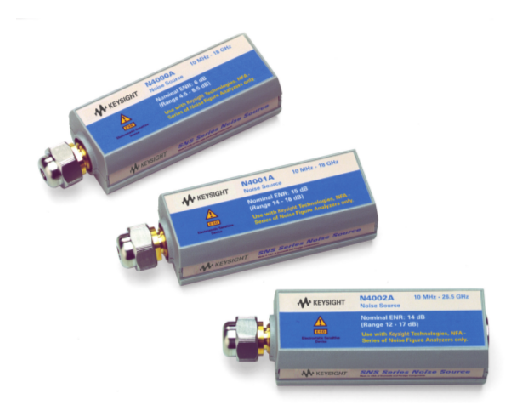
\includegraphics[width=8cm]{Imagenes/FuenteRuidoSNS.pdf}
		\caption{Fuente de ruido inteligente (SNS) de la serie N4000}
		\label{Fig:FuenteRuidoSNS}
	\end{figure}
	
	Las fuentes de ruido empleadas en su sistemas de calibración requieren de una fuente de ruido que entregue una señal con características plenamente conocidas, estandarizadas, estables. En el sistema de la figura \ref{Fig:BancoPruebasFuenteRuido} pueden emplearse dos series de modelos de fuentes de ruido, los modelos de la serie 346 y las fuentes de ruido inteligentes de la serie N4000, como se aprecia en la figura \ref{Fig:ModelosFuenteRuido}. Éstas últimas son las fuentes de ruido con las que cuenta el CENDIT.
	
	\begin{figure}[h!]
		\centering
		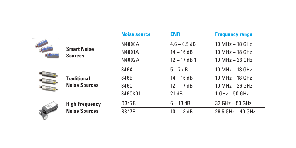
\includegraphics[width=15cm]{Imagenes/TablaFuentesRuido.pdf}
		\caption{Modelos para fuentes de ruido series 346 y N4000}
		\label{Fig:ModelosFuenteRuido}
	\end{figure}
	
	\subsection{Modo de operación}
	Las fuentes de ruido de la serie N4000 emplean un diodo semiconductor de silicio con polarización inversa como elemento generador de ruido de banda ancha. El nivel de potencia de ruido a la salida de la fuente es una función de la corriente inversa de polarización en el diodo. Las fuentes de ruido de la serie N4000 generan una señal de ruido con dos niveles de potencia distintos, conocidos como el \emph{nivel encendido (ON)} y el \emph{nivel apagado (OFF)}. 
	
	El nivel OFF ocurre cuando se elimina la corriente de inversa en el diodo, la fuente genera ruido debido a la agitación térmica de sus componentes internos con un nivel de potencia acorde a la temperatura física de la fuente. Se modela matemáticamente como ruido térmico de banda ancha, proporcional a la resistencia de salida de la fuente de ruido y la temperatura física de la misma. 
	
	El nivel ON sucede cuando se aplica la corriente de polarización inversa al diodo, el ruido a la salida se incrementa de manera sustancial. En este estado, la fuente aún genera el ruido térmico pero agrega una componente adicional de ruido, conocida como ruido en exceso. El ruido en exceso no es de naturaleza térmica, no depende de la temperatura física de la fuente, pero puede modelarse matemáticamente como tal por medio de la temperatura equivalente de la fuente de ruido.
	
	Las características de salida para una fuente de ruido vienen dadas en función de su rango de frecuencia y el nivel de potencia de ruido que entregan a su salida, expresada por la razón de ruido en exceso (ENR). Las fuentes de ruido de la serie N4000 poseen valores de nominales de ENR en el rango de 6 a 15 \si{\dB} para frecuencias entre 10 \si{\mega\hertz} y 26.6 \si{\giga\hertz}, tal como se indica en la tabla \ref{Tab:RangosFuentesRuido}.
	
	Los valores de ENR son calibrados en puntos específicos de frecuencia.
	
	\begin{table}[h!]
		\centering
		\begin{tabular}{cccc}
			\toprule
			Modelo de NS	&	ENR nominal (\si{\decibel})	& Rango de ENR (\si{\decibel})	&	Rango de frecuencia			\\
			\midrule	
			N4000A 	&	6.0	&	4.5 - 6.5	&	10 \si{\mega\hertz} - 18 \si{\giga\hertz} \\
			\midrule				
			N4001A 	&	15.0	&	14 - 16	&	10 \si{\mega\hertz} - 18 \si{\giga\hertz} \\
			\midrule	
			N4002A 	&	16.0	&	12 - 17	&	10 \si{\mega\hertz} - 26.5 \si{\giga\hertz} \\
			\bottomrule			
		\end{tabular}
		\caption{Rangos de ENR nominal para fuentes de ruido serie N4000}
		\label{Tab:RangosFuentesRuido}
	\end{table}
	
	Se emplean fuentes de ruido con bajo valor de ENR para minimizar el error por la no linealidad del detector de ruido. El error sera menor si la medida se realiza sobre un rango menor, en la zona de mayor linealidad, del detector de ruido. En este caso se emplea una fuente con ENR de 6 dB. [3]
	
	Estos dos niveles de ruido, ON y OFF, se usan para medición de ganancia y ruido agregado por parte del dispositivo bajo prueba, y por consiguiente, su figura de ruido.	
	
	\subsection{Estructura interna}
			
	En la figura \ref{Fig:DiagramaBloquesFuenteRuido} se muestra un diagrama de bloques que muestra la estructura interna de las fuentes de ruido de la serie N4000. La fuente de ruido requiere de una tensión de alimentación de +28 \si{\volt} para su operación. En las fuentes de ruido N4000A y N4001A, un inversor de voltaje interno convierte esta tensión a -25 \si{\volt} y la aplica al regulador de corriente que alimenta al bloque regulador de corriente para alimentar al diodo generador de ruido. El modelo N4002 emplea una polarización positiva, así que no posee un inversor de voltaje en su interior.
	
	El bloque regulador de corriente se encarga además de realizar la conmutación necesaria para producir los estados de ruido ON y OFF. Cuando se polariza el diodo de forma inversa, éste produce ruido de banda ancha el cual se inyecta al atenuador. El atenuador fija el valor final de ENR y establece la impedancia de salida de la SNS. Este atenuador es de 16 dB en los modelos N4000A para entregar a  su salida un ENR de 5 dB. Los modelos de SNS N4001A y N4002A utilizan un atenuador de 6 dB para entregar un valor nominal de ENR de 15 dB.		

	Los valores de ENR son dados en puntos de frecuencia cardinales sobre el rango de frecuencia de cada fuente, las parejas de datos frecuencia/ENR están almacenado en una EEPROM interna así como también los datos de incertidumbre y el coeficiente de reflexión complejo en ambos estados ON y OFF, documentados en el reporte de calibración. [1.8]. El ENR relaciona el nivel de ruido en exceso al ruido obtenido con la temperatura estándar de 296 K o al nivel de ruido que existe a la temperatura a estándar de 296 K. El valor de ENR no incluye la componente de ruido en OFF. 
	
	Las fuentes de ruido SNS poseen en su interior memoria EEPROM no volátil, en esta memoria residen los datos que caracterizan a una fuente de ruido particular en función de la frecuencia, como lo son el ENR y el coeficiente de reflexión, además de que incluyen modelo, numero de serial y la configuración de la intensidad de corriente de diodo y datos de calibración. Estos datos son almacenados  durante la calibración en fabrica de cada NS. Se encuentran dentro de un archivo en formato de texto plano, el incluye una tabla con filas de valores valores para ENR, coeficiente de reflexión con sus respectivas incertidumbres para puntos cardinales de frecuencia, distribuidos de manera uniforme sobre el rango de operación de la fuente de ruido. 	

	El NFA puede descargar los datos de ENR y coeficiente de reflexión, leerlos y modificarlos, para emplearlos en los cálculos de figura de ruido. Es por esta razón que esta fuentes se conocen como "inteligentes".	
	
	Las NS de la serie N4000 cuentan con un termómetro digital, se encuentra térmicamente acoplado al ensamble de microondas y le permita registrar la temperatura ambiente. EL NFA puede leer el valor de temperatura ambiente de este termómetro, lo emplea en los cálculos de figura de ruido en donde se necesite el valor de la temperatura fria, 			

	
	\begin{figure}[h!]{18}
		\centering
		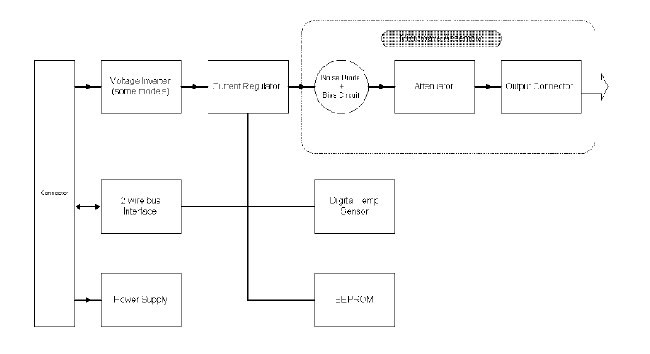
\includegraphics{Imagenes/DiagramaBloquesFuenteRuido.pdf}
		\caption{Diagrama de bloques para una fuente de ruido serie N4000}
		\label{Fig:DiagramaBloquesFuenteRuido}
	\end{figure}
	

	\subsection{Interfaces}
	Las fuentes de ruido inteligentes disponen de dos interfaces de tipo eléctrico: un interfaz de señal de RF y {\textmu}F y otra interfaz para comunicación de datos. 
	
	\subsubsection{Interfaz eléctrica: señal de ruido}
	Las características de las fuentes de ruido se determinan por tres parámetros. El más importante de estos es su \emph{razón de ruido excedente (ENR)}, la cual indica, de forma indirecta, la potencia de ruido nominal que la fuente puede entregar. Viene dada por una razón de potencias de ruido o de temperaturas de ruido equivalentes, es una cantidad adimensional, pero es practica común expresarla en decibelios. En la tabla \ref{Tab:RangosNominalesENR} se indican los niveles nominales para las fuentes de ruido de las series 346 y N4000.
	
	\begin{table}[h!]
		\centering
		\begin{tabular}{cc}
			\toprule
			Modelo de NS	&	Rango de ENR (\SI{}{\decibel})		\\
			\midrule	
			N4000A / 346A	&	4.5 - 6.5 					\\
			\midrule				
			N4001A / 346B	&	14 - 16  					\\
			\midrule	
			N4002A / 346C	& 	12 - 17 					\\
			\bottomrule			
		\end{tabular}
		\caption{Rangos de ENR nominal para fuentes de ruido}
		\label{Tab:RangosNominalesENR}
	\end{table}

	Los dos parámetros restantes que describen una fuente de ruido están relacionados con el acople con el resto del sistema, estos son el ROE (SWR) y su coeficiente de reflexión. Los tres parámetros descriptivos, el ENR, la ROE y el coeficiente de reflexión son dependientes de la frecuencia. En la tabla \ref{Tab:CaracteristicasElectricasN4000} se resumen estos datos para las fuentes de ruido de la serie N4000 para los rangos de frecuencia respectivos a cada modelo de fuente de ruido.
	
	\begin{table}[h!]
		\centering
		\begin{tabular}{cccc}
				\toprule
					& Rango de frecuencia & ROE máxima & Coeficiente de reflexión 	\\
					& (\si{\giga\hertz})  &			   & para los estados ON / OFF	\\
				\midrule
			N4000A	&	0.01 - 1.5	&	< 1.06 : 1	&	0.03	\\
					&	1.5	- 3.0	&	< 1.06 : 1	&	0.03 	\\
					&	3.0 - 7.0	&	< 1.13 : 1	&	0.06	\\
					&	7.0	- 18.0	&	< 1.22 : 1	&	0.10	\\
				\midrule
			N4001A	&	0.01 - 1.5	& 	< 1.15 : 1 	&	0.07	\\
					&	1.5 - 3.0	&	< 1.15 : 1	& 	0.07	\\
					& 	3.0 - 7.0	& 	< 1.20 : 1	&	0.09	\\
					&	7.0	- 18.0	&	< 1.25 : 1	&	0.11	\\
				\midrule
			N4002A	&	0.01 - 1.5	&	< 1.22 : 1	& 	0.10	\\
					&	1.5	- 3.0	&	< 1.22 : 1	&	0.10	\\
					&	7.0	- 18.0	&	< 1.25 : 1	&	0.11	\\
					&	18.0 - 26.5	&	< 1.35 : 1	&	0.15	\\
				\bottomrule			
		\end{tabular}
		\caption{Características eléctricas para fuentes de ruidos SNS serie N4000}
		\label{Tab:CaracteristicasElectricasN4000}
	\end{table}
	
	\begin{table}[h!]
		\centering
		\begin{tabular}{cccc}
			\toprule
			Modelo de SNS		&	N4000A		&	N4001A		&	N4002A	\\
			\midrule
			Rango de frecuencia	&	\SI{10}{\mega\hertz} a \SI{18}{\giga\hertz} & \SI{10}{\mega\hertz} - \SI{18}{\giga\hertz} & \SI{10}{\mega\hertz} - \SI{18}{\giga\hertz} \\
			\midrule
			Conector			&	\multicolumn{3}{c}{APC \SI{3.5}{\milli\meter} con opción de Tipo-M (m)}	\\
			\midrule
			ENR nominal	(\si{\decibel})		&	6 		&	6		&	30		\\
			\midrule
			Rango de ENR (\si{\decibel}) 	& 4.5 - 6.5 & 14 - 16	& 12 - 17 	\\
			\midrule
			Rango de F en el DUT (\si{\decibel}) & < 20		& < 30 		& 	?	 \\
			\midrule
			Rango de temperatura (\si{\degreeCelsius}) 	& \multicolumn{3}{c}{0 a 55} \\
			\midrule
			Precisión 				& \multicolumn{3}{c}{$\pm 1 a \SI{25}{\degreeCelsius}$} \\
									& \multicolumn{3}{c}{$\pm 2 de 0 a \SI{55}{\degreeCelsius}$} \\
			\midrule
			Impedancia (\si{\ohm})  & \multicolumn{3}{c}{ 50 } \\
			\midrule
			Máxima potencia inversa (\si{\watt}) 	& \multicolumn{3}{c}{1} \\
			\midrule
			Variación de ENR con temperatura 		& \multicolumn{3}{c}{ < \SI{0.01}{\decibel} / \si{\degreeCelsius} de \SI{30}{\mega\hertz} a \SI{26}{\giga\hertz}} \\
			\midrule
			Sensor de temperatura 	& Rango 		& \multicolumn{2}{c}{0 a \SI{55}{\degreeCelsius}} \\
									& Resolución 	& \multicolumn{2}{c}{\SI{0.25}{\degreeCelsius}} \\
									& Precisión 	& \multicolumn{2}{c}{$\pm \SI{1}{\degreeCelsius} a \SI{25}{\degreeCelsius}$} \\
									&				& \multicolumn{2}{c}{$\pm \SI{2}{\degreeCelsius} de 0 a \SI{55}{\degreeCelsius}$} \\ 
			\bottomrule									
		\end{tabular}
	\end{table}	
	


	Los valores de ENR son dados en puntos de frecuencia cardinales sobre el rango de frecuencia de cada fuente, las parejas de datos frecuencia/ENR están almacenado en una EEPROM interna así como también los datos de incertidumbre y el coeficiente de reflexión complejo en ambos estados ON y OFF, \ documentados en el reporte de calibración. [1.8]. El ENR relaciona el nivel de ruido en exceso al ruido obtenido con la temperatura estándar de 296 K o al nivel de ruido que existe a la temperatura a estándar de 296 K. El valor de ENR no incluye la componente de ruido en OFF. 
	
	\subsubsection{Interfaz de comunicaciones}
	Las fuentes de ruido almacenan los datos de calibración en su memoria EEPROM interna y poseen un termómetro digital, el NFA N8975 cuenta con la capacidad para descargar estos datos de calibración y leer el valor de temperatura, para luego emplearlos en los cálculos de figura de ruido.
	
	La transferencia de datos entre la fuente de ruido y el NFA se realiza a través de un bus serial (two-wire bus). 
	
	El NFA debe proveer una alimentación de +5 V a la interfaz serial, la memoria EEPROM y el sensor digital de temperatura. Las fuentes de ruido SNS utiliza emplean un bus serial (two-wire bus) para transferencia de datos entre la fuente de ruido y el NFA. 
	
	\subsection{Selección de fuente de ruido}
	Se emplean fuentes de ruido con bajo valor de ENR para minimizar el error por la no linealidad del detector de ruido. El error sera menor si la medida se realiza sobre un rango menor, en la zona de mayor linealidad, del detector de ruido. En este caso se emplea una fuente con ENR de 6 dB.
	
	Se debe emplear una fuente de ruido con un conector adecuado para el DUT en vez de emplear un adaptador, en especial para dispositivos de alta ganancia. Los valores de ENR para una fuente de ruido aplican solo hasta el su conector. Un adaptador añade perdidas a los valores de ENR, la incertidumbre en estas perdidas incrementa la  total en la medición. Si se usa un adaptado, se deben tomar en cuenta sus perdidas. [3].
	
	Es importante emplear un NS con el menor cambio en su impedancia de salida entre sus estado de encendido y apagado. Estos cambios de impedancia alteran el acoplamiento entre la NS y el DUT lo que conlleva a cambos en la ganancia y en la figura de ruido del DUT. Las fuentes de ruido comerciales de 6dB ENR limitan el cambio del coeficiente de reflexión entre los estados ON y OFF a menos de 0.01 a frecuencias hasta de 18 GHz. [3]
	
	Las fuentes de ruido con bajo valor de ENR son ideales para medición, sin embargo, las fuentes de alto ruido son necesarias para calibrar el rango dinámico completo del instrumento. Los NFA pueden tomar en cuenta las distintas tablas de ENR requeridas para la calibración y medida. [3]
	
	Una fuente con un bajo valor de ENR necesitara en el instrumento un menor valor de atenuación para cubrir el rango dinámico, excepto cuando la ganancia del DUT es muy alta. Emplear menor atenuación redice la figura de ruido del instrumento de medición, lo cual a su vez reduce la incertidumbre en la medición. [3]	
	
	%\subsection{Controlador de interruptores y atenuadores 11713 (Attenuator Switch Driver)}
Los equipos de la serie 11713 están diseñados para generar las señales de control o conmutación para bancos de atenuadores o interruptores electromecánicos para RF y \textmu, de acuerdo a la selección hecha por el usuario en su panel frontal o en forma de comando enviado de forma remota a este dispositivo a través de un bus GPIB, USB o una red LAN.
Los atenuadores e interruptores coaxiales electromecánicos que no dispongan de interfaz de usuario, se debe emplear un equipo de la serie 11713 para que el usuario pueda controlar a estos dispositivos.

El 11713 permite al usuario controlar un banco de interruptores o atenuadores interactuando con su interfaz física en su panel frontal (modo local) y también permite control en modo remoto, el usuario puede enviar comandos a través de un bus GPIB (modelo 11713A), un bus USB o una red LAN (modelos 111713B y 11713C).

Fabricado inicialmente por Agilent Technologies con el modelo 11713A (figura \ref{Fig:Versiones11713}a) actualmente es producido por Keysight Technologies, en dos versiones mejoradas pero que conservan toda la funcionalidad del equipo original de Agilent, en los equipos 11713B (figura \ref{Fig:Versiones11713}b) y 11713C (figura \ref{Fig:Versiones11713}c).

\begin{figure}[h!]
{
	\centering
	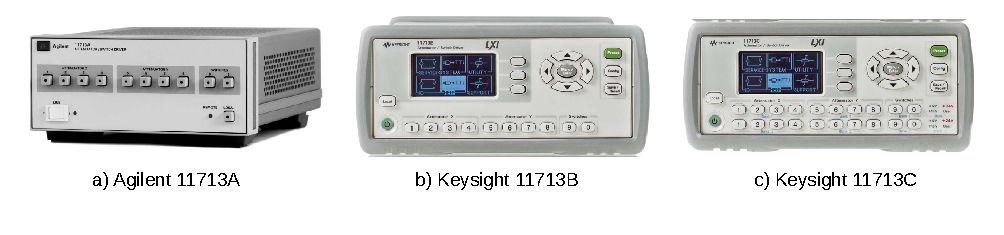
\includegraphics[width=\textwidth]{./Imagenes/Versiones11713.pdf}
	\caption{Versiones para los equipos de la serie 11713.}
	\label{Fig:Versiones11713}
}
\end{figure}

Los equipos de la serie 11713 pueden controlar una amplia gama de modelos de atenuadores o interruptores, en la tabla \ref{Tab:ModelosInterruptoresAgilent} se muestran los modelos compatibles de Agilent. Los interruptores a controlar pueden ser de tipo
SPDT, bypass, matrix, transfer y multipuerto.


\begin{table}[h!]
	\centering
	\begin{tabularx}{\textwidth}{cX}
		\toprule
		Tipo de interruptor	&	Modelos \\
		\midrule
		SPDT 				&	8761B, 8762A/B/C/F, 8765A/B/C/D/F, N1810TL, N1810UL \\
		\midrule 
		Bypass				&	8763A/B/C, 8764A/B/C, N1811TL, N1812UL \\
		\midrule			
		Multipuerto			&	87104A/B/C, 87204A/B/C, 87106A/B/C, 87206A/B/C, 8766K, 8767K, 8768K, 8769K, 8767M, 8768M, 8769M \\
		\midrule
		Matrix				&	87406B, 87606B \\
		\midrule
		Transfer			& 	87222C/D/E \\
		\bottomrule
	\end{tabularx}
	\caption{Modelos de interruptores Agilent/Keysight compatibles con el 11713}
	\label{Tab:ModelosInterruptores11713}
\end{table}

\begin{table}[h!]
	\centering
	\begin{tabular}{cc}
		\toprule
		Modelo de atenuador	 	&	Atenuación 			\\		
		\midrule
		8494G,H (33320G,H)		&	11 dB, paso 1 dB	\\
		\midrule
		8495G,H,K (33321 G,H,K)	&	70 dB, paso 10 dB 	 \\
		\midrule
		8496G,H (33322G,H)		&	110 dB, paso 10 dB   \\
		\midrule		
		8497K ( 33323K)			&	90 dB, paso 10 dB 	 \\
		\midrule		
		84904K,L (33324K,L)		&	11 dB, paso 1 dB 	\\
		\midrule		
		84906K,L ( 33326K,L)	& 	90 dB, paso 10 dB 	\\
		\midrule		
		84907K,L (33327K,L) 	& 	70 dB, paso 10 dB 	\\
		\bottomrule		
	\end{tabular}
	\caption{Modelos de atenuador Agilent/Keysight compatibles con el 11713}
	\label{Tab:ModelosAtenuadores11713}
\end{table}
Los equipos de la serie pueden manejar un numero de atenuadores o interruptores, según el modelos. En general, el modelo 11713C puede el doble de atenuadores e interruptores que el modelo 11713B.

Los equipos de la serie 11713 disponen de dos tipos de interfaces, una interfaz de usuario y una interfaz eléctrica. Los equipos 11713B y 11713C agregan una tercera interfaz de comunicaciones. Estos equipos no presentan una interfaz para señales de RF o UW, no manejan ni realizan mediciones sobre este tipo de señales.

La interfaz de usuario se encuentra en el panel frontal de estos equipos, en el 11713A consiste básicamente en tres grupos de pulsadores. Los equipos 11713B y el 11713C también disponen de pulsadores en su panel frontal y además agregan una pantalla LCD a la interfaz de usuario.

\begin{table}[h!]
	\begin{tabularx}{\textwidth}{cXXXX}
		\toprule
			&	&	11713A	&	11713B	&	11713C \\
		\midrule
		\multirow{5}{*}{Botones} & Control de \newline atenuadores X & 1 panel de 4 botones & 1 panel de 4 botones & 2 paneles de 4 c/u. \\
			&	Control de \newline atenuadores Y & 1 panel de 4 botones & 1 panel de 4 botones & 2 paneles de 4 c/u. \\
			& 	Control de \newline interruptores & 1 panel de 2 botones &  1 panel de 2 botones & 2 paneles de 2 botones c/u. \\
			& 	Teclas de flecha 	&	No	& Si	& Si \\
			& 	Preset, Config, Save/Recall	& No	&	Si	& Si \\
		\midrule
		Pantalla LCD	& No	& Si	& Si
	\end{tabularx}
	\caption{Características de interfaz de usuario en los equipos 11713}
	\label{Tab:CaracteristicasInterfazUsuario11713}
\end{table}


El 11713 presenta una interfaz eléctrica la cual entrega señales de control que permiten seleccionar un nivel de atenuación en los atenuadores o abrir y cerrar un interruptor coaxial. Esta interfaz es accesible por medio del panel trasero de los equipos de la serie 11713, en forma de conectores como se aprecia en la figura 8 un detalle del panel posterior del 11713B. En este panel se encuentran los conectores con las señales de control para atenuadores e interruptores coaxiales. 

\begin{table}[h!]
	\begin{tabularx}{\textwidth}{XXXX}
		\toprule
				& 11713A	& 	11713B	&	11713C \\
		\midrule
		Control de atenuadores (pares de conector Viking de 12 pines)	& 1 par & 1 par & 2 pares \\
		\midrule
		Control de interruptores coaxiales (pares de jacks banana)	& 1 par (A y B) & 1 par (A y B) & 2 pares (A y B) \\
		\midrule
		Alimentación DC en los puertos & +24 V DC & +24 V DC +5, +15, +24 V DC, ajustable por usuario \\
		\midrule
		Control TTL & No & No & Si \\
		\midrule
		Cantidad máxima de atenuadores & 2 de 4 secciones & 2 de 4 secciones & 4 \\
		\midrule 
		Cantidad máxima de interruptores & 2 en los jacks banana. Hasta 10 SPDT en los conectores Viking & 4 en los jacks banana. Hasta 10 SPDT en los conectores Viking & 2 en los jacks banana. Hasta 20 SPDT en los conectores Viking. \\
		\bottomrule
	\end{tabularx}
	\caption{Interfaz eléctrica en los equipos 11713}
	\label{Tab:Interfaz eléctrica en los equipos 11713}
\end{table}

En un banco de atenuadores, como los de Agilent, la cantidad de atenuación que se introduce en el camino de señal es determinada por apertura o cierre de un un conjunto de interruptores electromecánicos, que insertan o retiran atenuadores en el camino de señal. Los interruptores coaxiales también emplean interruptores electromecánicos. Las
señales de comando que el 11713 envía a los interruptores electromecánicos es una señal de potencia, de tipo lógico y referidas a tierra.

Las señales de control para los modelos de atenuadores Agilent se encuentran en los conectores Viking. Existe un par de éstos en los modelos 11713 A y B, etiquetados como ATTEN X y ATTEN Y. El modelo 11713C dispone de dos pares de conectores Viking. Las señales presentes en los conectores Viking también pueden emplearse para el control de interruptores electromecánicos coaxiales.

La conexión entre un equipo de la serie 11713 con un atenuador o un interruptor coaxial se realiza por medio de cables especiales que se insertan en los conectores que disponen estos equipos. La información sobre modelos de cable de acuerdo al modelo de atenuador o interruptor se ofrece en las hojas de datos en forma de matrices de selección. Los
cables de conexión se eligen de acuerdo al numero de opción de los equipos 11713 y de acuerdo al modelo del equipo atenuador o interruptor, ubicando estos datos en la matriz de selección. La matriz de selección remite a una figura en donde se indica un esquema con instrucciones para realizar las conexiones entre éstos equipos. 

\begin{figure}[h!]
	\centering
	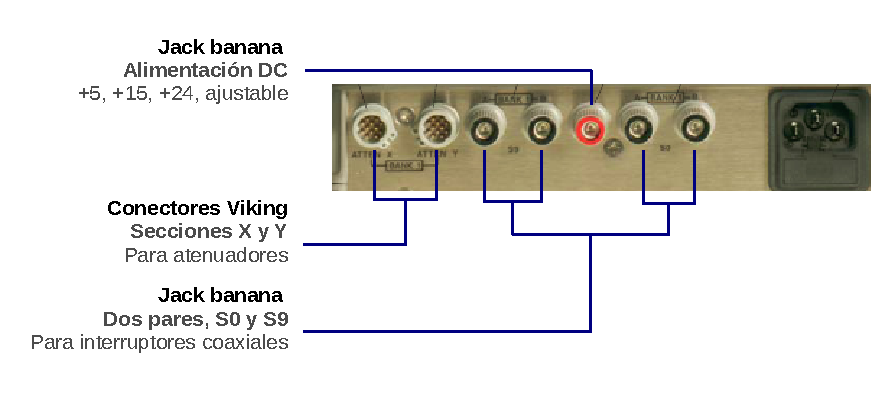
\includegraphics[width=0.8\textwidth]{Imagenes/SeccionPanelPosterior11713.pdf}
	\caption{Sección del panel posterior del 11713B}
	\label{Fig:SeccionPanelPosterior11713}
\end{figure}

Existe un modelo de cable apropiado para cada modelo de atenuador o interruptor coaxial, pero uno de sus extremos siempre debe poseer un conector Viking hembra si se desean utilizar éstos con un equipo 11713. 

\ Un conector Viking en el equipo 11713, como se muestra en la figura \ref{seq:refDrawing8}, \ posee 12 pines. Los pines 1 y 2 portan la tensión DC para alimentar al periférico. Esta tensión de alimentación DC en los equipos 11713A y
11713B es de valor fijo de +24 V DC, en el 11713C puede ser seleccionada por el usuario a un valor fijo de +5, +15, +24 V DC o ajustada a un valor entre 0 y +24 V DC. Los pines del 3 al 12 llevan las señales de conmutación, las cuales son de tipo lógico. En la figura \ref{seq:refDrawing9} se muestra un esquema de driver interno en el 11713 para las señales
de control. De esta figura se deduce que las señales de control trabajan en pares, esto es, mientras un pin es llevado a tierra el pin complementario es colocado en alta impedancia. Las señales de control en conjunto con la alimentación DC común permite manejar parejas de interruptores electromecánicos en dos estados, abierto y cerrado, o interruptores electromecánicos simples en los cuales una bobina abre y otra bobina cierra el circuito.

\begin{figure}[h!]
	\centering
	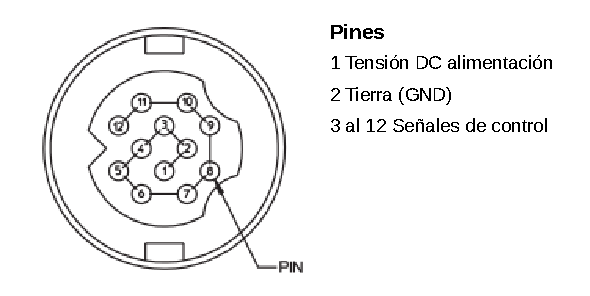
\includegraphics[width=0.6\textwidth]{Imagenes/PinoutConectorViking.pdf}
	\caption{Descripción de pines de un conector Viking}
	\label{Fig:PinoutViking}
\end{figure} 

\begin{figure}[h!]
	\centering
	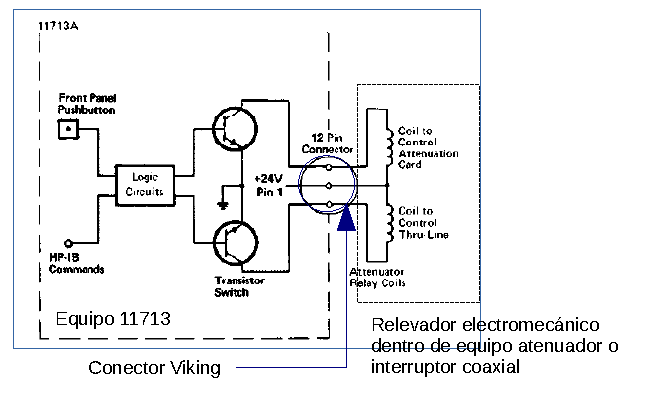
\includegraphics[width=0.8\textwidth]{Imagenes/DiagramaInternoConectorViking.pdf}
	\caption{Diagrama interno generación de señales en conectores Viking}
	\label{Fig:DiagramaInternoConectorViking}
\end{figure}

Los conectores banana ubicados en el panel posterior en los equipos 11713 (figura 8) están destinados al comando de interruptores electromecánicos coaxiales. Están dispuestos en parejas y etiquetados como A y B. En los  modelos 11713A y 11713B existen dos pares de éstos (S0 y S9) y en el modelo 11713C posee cuatro pares con las etiquetas S0 y S9 (Bank1 y Bank2). En la figura 11 se muestra un diagrama del driver interno para estos puertos. Ambos jacks bananas, A y B, generan una señal de tipo binaria y trabajan de forma complementaria, esto significa que cuando un jack presenta la tensión de tierra (0 V) el jack complementario presenta una tensión DC. Cada grupo de conectores S0 y S9 disponen de un jack banana común con un suministro de alimentación DC, para los interruptores que la requieran. Esta tensión de alimentación en los equipos 11713A y 11713B es fija en +24 V DC. En el modelo 11713C esta tensión es puede ser programada por el usuario a un valor fijo de +5, +15 y 25 VDC o ajustada a un valor entre 0 y +24V DC.

\begin{figure}[h!]
	\centering
	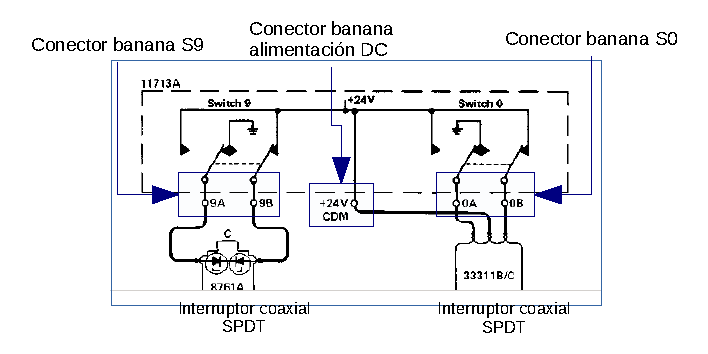
\includegraphics[width=0.8\textwidth]{Imagenes/DiagramaInternoJackBanana.pdf}
	\caption{Diagrama interno generación de señales en jack banana}
	\label{Fig:DiagramaInternoJackBanana}
\end{figure}

En el sistema para medición de ruido de la figura 1, un equipo de la serie 11713 se emplea con un doble propósito, servir como interfaz de usuario y controlador del banco de atenuadores N2002. El estado de cada pareja de pines en un conector Viking en el panel posterior de estos equipos esta relacionado en forma directa con el estado del un botón en el panel frontal. En la tabla 2 se indica esta relación. Los botones en el panel frontal ubicados en la sección etiquetado como Attenuator X controlan el estado de los pines ubicados en el conector Viking del panel posterior etiquetado como ATTEN X. Se cumple una relación idéntica para los botones en la sección etiquetada como Attenuator Y del panel frontal y los conectores Viking etiquetados como ATTEN Y del panel posterior. Por ejemplo los pines 5 y 6 en el conector Viking ATTEN X se corresponde al estado del botón 1 en la sección Attenuator X. De la misma forma, los pines 5 y 6 del conector Viking ATTEN Y responden al estado del botón 5 de la sección Attenuator Y.

\begin{table}[h!]
	\centering
	\begin{tabular}{cc}
		\toprule
		\textbf{Pines} 				&	\textbf{Controlado por botones}			\\
		\textbf{ATTENX y ATTEN Y}	&	\textbf{Attenuator X, Attenuator Y} 	\\
		\midrule
		1	&	Alimentación 	\\
		\midrule
		2	&	Tierra 			\\
		\midrule		
		5	&	\multirow{2}{*}{Botón 1 para ATTEN X Botón 5 para ATTEN Y} \\
		6	&																		\\
		\midrule		
		7	&	\multirow{2}{*}{Botón 2 para ATTEN X Botón 6 para ATTEN Y}	\\
		8	&																		\\
		\midrule		
		9	&	\multirow{2}{*}{Botón 3 para ATTEN X Botón 7 para ATTEN Y}	\\	
		10	&													 					\\
		\midrule		
		11	&	\multirow{2}{*}{Botón 4 para ATTEN X Botón 8 para ATTEN Y}	\\
		12	&																		\\ 
																						 														
		\bottomrule		 
	\end{tabular}
	\caption{Relación de botones panel frontal con los pines en puertos Viking}
	\label{Tab:RelacionBotonesPuertosViking11713}
\end{table}

Los pines en los puertos Viking operan en pareja y de forma complementaria, cuando un pin se encuentra a tierra (GND) su pareja correspondiente se encuentra en alta impedancia. En la tabla 3 se indica la relación que existe  entre el estado de los botones en el panel frontal y el estado de los pines en los conectores Viking. Por ejemplo, cuando el botón 1 del panel Attenuator X se encuentra encendido, en el respectivo conector Viking ATTEN X, el pin 5 se encuentra a tierra (GND) mientras que su pin complementario se encuentra en alta impedancia. Cuando el mismo botón se apaga, los pines 5 y 6 intercambian de estado.

\begin{table}[h!]
	\centering
	\begin{tabular}{ccccc}
		\toprule
		\multicolumn{2}{c}{\bfseries Botones Attenuators} &
		\multirow{2}{*}{\bfseries Estado del botón} & 
		\multicolumn{2}{c}{\bfseries Pines puerto ATTEN} \\
		X & Y &			& Pin & Estado \\
		\midrule
		\multirow{4}{*}{1} & \multirow{4}{*}{5} 
			& \multirow{2}{*}{OFF}    & 5 & GND		\\
			&  &                      & 6 & Hi-Z	\\
			&  & \multirow{2}{*}{ON}  & 5 & Hi-Z	\\
			&  &                      & 6 & GND		\\
		\midrule			
		\multirow{4}{*}{2} & \multirow{4}{*}{6} 
		& \multirow{2}{*}{OFF}    & 7 & GND		\\
		&  &                      & 8 & Hi-Z	\\
		&  & \multirow{2}{*}{ON}  & 7 & Hi-Z	\\
		&  &                      & 8 & GND		\\
		\midrule			
		\multirow{4}{*}{3} & \multirow{4}{*}{7} 
		& \multirow{2}{*}{OFF}    &  9 & GND		\\
		&  &                      & 10 & Hi-Z	\\
		&  & \multirow{2}{*}{ON}  &  9 & Hi-Z	\\
		&  &                      & 10 & GND	\\		
		\midrule			
		\multirow{4}{*}{4} & \multirow{4}{*}{8} 
		& \multirow{2}{*}{OFF}    & 11 & GND		\\
		&  &                      & 12 & Hi-Z	\\
		&  & \multirow{2}{*}{ON}  & 11 & Hi-Z	\\
		&  &                      & 12 & GND	\\				
		\bottomrule
	\end{tabular}
	\caption{Configuracion de botones y su relación con el estado de los pines en los uertos Viking}
	\label{Tab:RelacionBotonesEstodoPinesViking11713}
\end{table}

Los jack banana presentes en el panel posterior, etiquetados como A y B bajo las secciones S9 y S0, también operan por parejas, su estado es complementario y es función del estado presente en los botones del panel frontal, etiquetados como S9 y S0. La tabla 4 resume la relación que existe entre los botones S9 y S0 con los niveles de tensión presentes en los jack banana A y B de las secciones S9 y S0. Por ejemplo, de la tabla 4 se observa que cuando el botón S9 esta encendido (ON), en la sección S9 del panel posterior el estado el jack banana A  se encuentra puesto a tierra (0 V) mientras que el jack banana B presenta una tensión positiva DC (+24 V en el 11713 A). Si ahora el botón S9 se apaga (OFF), los jacks banana A y B de la sección S9 intercambian de estado.

\begin{table}[h!]
	\begin{tabular}{|c|c|c|c|c|}
		\hline
		\multirow{2}{*}{\bfseries Interruptor coaxial} & \multirow{2}{*}{\bfseries Estado botones S9 y S0} & \multicolumn{3}{c}{\bfseries Tensión jack banana panel posterior} \\
		\cline{3-5}
			& 	&	\textbf{Jack}	&	\textbf{A}	&	\textbf{B}  \\
		\hline
		\multirow{2}{*}{S9} & OFF 	& S9 	& +\si{\volt} DC 	& GND \\
		\cline{2-5}
							& ON	& S9	& GND				& +\si{\volt} DC \\
		\hline
		\multirow{2}{*}{S0} & OFF 	& S0 	& +\si{\volt} DC 	& GND \\
		\cline{2-5}
							& ON	& S0	& GND				& +\si{\volt} DC \\
		\hline								
		
	\end{tabular}
	\caption{Relación entre los botones S9 y S0 en el panel frontal y los jacks banana en el panel posterior}
	\label{Tab:RelacionBotonesJackBanana11713}
\end{table}]

En el sistema para medición de figura de ruido, el banco de atenuadores N2002 permite el paso de ciertos intervalos de frecuencia de acuerdo al estado de los botones en el panel frontal de un equipo de la serie 11713.   En la tabla 5 se muestran los rangos de frecuencia de las señales para las cuales el N2002 permite el paso en función del estado de los botones en las secciones Attenuator X y Attenuator Y del panel frontal de un 11713. De esta tabla, cuando los interruptores S9 y S0 están presionados, el N2002 admite el paso de señales cuyas frecuencias se encuentre entre 10 MHz y 3 GHz. Cuando los botones 1 y 5 de las secciones respectivas Attenuator X y  Attenuator Y del panel frontal están presionados, el N2002 admite el paso de señales con frecuencias comprendidas entre 3 GHz y 6 GHz.

\begin{table}[h]
	\centering
	\begin{tabularx}{0.6\textwidth}{|c|c|c|c|c|c|c|c|c|c|c|}
		\hline
		\multirow{3}{*}{\bfseries Rango de frecuencia} &
		\multicolumn{8}{c}{Atenuadores} & 
		\multicolumn{2}{c}{\multirow{2}{*}{Interruptores}} \\	
				& \multicolumn{4}{c}{\bfseries Attenuator X} 
				& \multicolumn{4}{c}{\bfseries Attenuator Y} \\
		\cline{2-11}				
				  						& 1 & 2 & 3 & 4 & 5 & 6 & 7 & 8  & S9 & S0 \\
		\hline
		10 a < 3000 \si{\mega\hertz}    &   &   &   &   &   &   &   &    &  X &  X \\
		3 a 6 \si{\giga\hertz} 			& X &   &   &   & X &   &   &    &    &    \\
		< 6 a 12 \si{\giga\hertz}		&   &   & X &   &   &   & X &    &    &    \\				
		> 12 a 18 \si{\giga\hertz}		&   & X &   &   &   & X &   &    &    &    \\
		> 18 a 26.5 \si{\giga\hertz}	&   &   &   & X &   &   &   & X  &    &    \\	
		
		\hline
		
	\end{tabularx}
	\caption{Relación entre los rangos de frecuencia de paso de banda en el N2002 y la combinación de botones en un equipo 11713}
	\label{Tab:ControlRangoFrecuencia11713}
\end{table}
	
	
	%\subsection{Analizador de figura de ruido N8975A (NFA Series Noise Figure Analyzer)}
\subsubsection{Descripción general}

Representa el equipo fundamental en el sistema de la figura 2, es esencialmente un dispositivo que mide de potencia de ruido en RF y UW generada por elementos pasivos o activos. A partir de la medida de potencia, este equipo puede	calcular el valor de la figura de ruido de elemento, así como también su temperatura efectiva, ganancia y presentar el resultado en pantalla. 

El NFA mide la potencia total de ruido que genera un dispositivo bajo prueba (DUT por sus siglas en inglés) cuando en su entrada se inyecta una señal de ruido de referencia. Esta señal es producida por una fuente de ruido estándar, sus características de ruido deben ser conocidas con elevada exactitud. En el sistema CENDIT, se emplean las fuentes de ruido de la serie Agilent N4000A. La fuentes de ruido N4000A son conocidas como fuentes de ruido inteligentes, ya que	estas almacenan en una memoria no volátil interna, una tabla que caracteriza su potencia de ruido en función de la frecuencia, conocida como tabla de ENR. Además, cuentan con un sensor de temperatura integrado.

A través de un cable que conecta el NFA con el puerto de control de la NS, el NFA puede cargar las tablas de ENR de las fuentes de ruido. De la misma forma, puede leer la temperatura de la fuente de ruido.

\begin{figure}[h!]
	\centering
	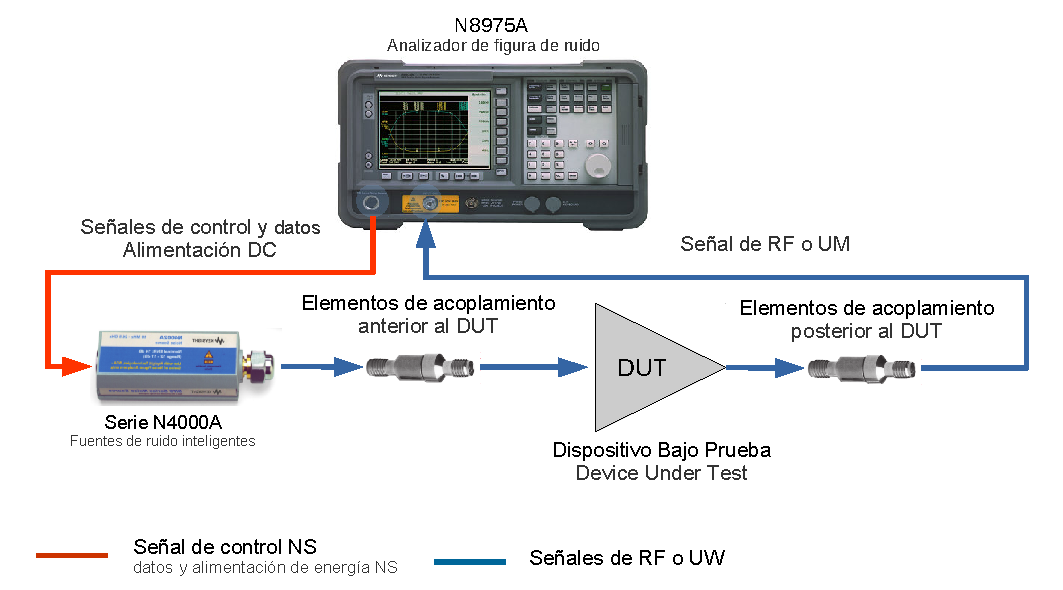
\includegraphics[width=15cm]{./Imagenes/EsquemaConexionNFADUT.pdf}
	\caption{Esquema de conexiones de la instrumentación básica para medición de NF.}
\label{Fig:BancoPruebasFuenteRuido}
\end{figure}

El N8975 emplea la técnica del factor Y para la medición de ruido sobre un DUT. Esta técnica consiste básicamente en	inyectar en la entrada del DUT dos niveles distintos de potencia de ruido, el primero   sensiblemente mayor que el segundo, para luego medir la potencia de ruido que a la salida del DUT existen para cada uno de estos niveles.	Calculado un cociente entre el valor mayor y el valor menor de la medición, esto es el factor Y, y con la tabla de	ENR de la fuente de ruido se puede conseguir la figura del ruido del DUT.

Aparte de la figura de ruido, puede realizar las siguientes mediciones:

\begin{itemize}
	\item Potencia de ruido, fría PCOLD y caliente PHOT
	\item Temperatura equivalente de ruido.
	\item Factor Y.
	\item Ganancia.
\end{itemize}

El NFA cuenta con las siguientes interfaces

\begin{itemize}
	\item Una interfaz de usuario, en su panel frontal. 
	\item Una interfaz de señal (RF y {}W)
	\item Una interfaz de datos.
\end{itemize}

La interfaz de usuario se divide a su vez en dos interfaces: interfaz local e interfaz remota. La interfaz local permite al usuario operar el NFA en sitio, la constituye el panel frontal del equipo el cual cuenta con una pantalla LCD y un conjunto de botones agrupados en bloques de acuerdo a su funcionalidad y un teclado numérico.

El monitor LCD es a color, de 17 cm, en el se presentan los datos ya se en formato de gráfico, tabla o modo de medidor.Puede presentar dos gráficas simultaneas, en estas se pueden agregar cuatro marcadores o cursores y dos lineas limites. Puerto paralelo, 25 pines D-sub, dedicado a impresora. Salida VGA conector 15 pines, mini D-sub, hembra.

El NFA dispone de la capacidad para ser operado de forma remota. En su panel trasero cuenta con un conector IEEE-488 para bus GPIB y un conector RS-232 D-sub de 9 pines. El conector IEEE-4888 permite conectar el equipo a un bus GPIB y establecer una red de instrumentos de medición. Es posible además conectar el puerto GPIN del NFA a un computador, por medio de una tarjeta como las del tipo PCI-GPIB y cable de bus GPIB empleando o un adaptador USB-GPIB. A través de bus GPIB y empleando aplicaciones de software se le envían comandos al equipo que permiten controlarlo y obtener datos de mediciones.

Interfaz GPIB conector IEEE-488, bus serial RS-232, 9 pines D-sub, macho.	
La interfaz de señal señal que dispone el equipo en su panel frontal consiste en 

\begin{itemize}
	\item Un conector de entrada para señal RF-$\mu${\textmu}F. 
	\item Un conector de salida para el control, alimentación y datos de una fuente inteligente de ruido (SNS) de la serie N4000 de Agilent 
	\item Un puerto para alimentación y conmutación de una fuente de ruido tradicional serie 346 de Agilent. 
\end{itemize}
EL conector de entrada para señal de RF / UW es de tipo APC 3.5 (m), con \ impedancia nominal de 50 Ω, ESD sensible. La potencia máxima admisible en la señal de entrada es de 10 dBm. La máxima protección de entrada ± 20V, +15dBm pico (o promedio) en RF. El rango de frecuencia admisible por ele equipo es de 10 a 26.5 GHz.

En el conector SNS se conecta una fuente de ruido SNS, a través de un cable multihilo cilíndrico. Por medio de este puerto el equipo enviá y recibe los datos almacenados de ENR y temperatura medida por la NS además de la señal de alimentación que permite conmutar la potencia de ruido generada por la SNS, las señales de alimentación y datos. 

\subsubsection{Interfaz eléctrica}

Rango de frecuencia: 10 a 26,5 GHz

Ancho de banda de medición: 4 MHz, 2 MHz, 1 MHz, 400 kHz, 200 kHz, 100 kHz.

El desempeño depende del ENR de la fuente empleada	

\begin{table}
	\centering
	\begin{tabular}{ccccc}
		\toprule
		\multicolumn{2}{c}{\bfseries Rango de ENR para la fuente   de ruido} &
		{\bfseries 4 - 7 \si{\decibel}} & 
		{\bfseries 12 - 17 \si{\decibel}} & 
		{\bfseries 20 - 22 \si{\decibel}} \\
		\midrule
		\multirow{2}{*}{\bfseries 10 \si{\mega\hertz} a 3 \si{\giga\hertz}} & {\bfseries Rango de medición} 
		& 0 a 20 \si{\decibel} 	& 0 a 30 \si{\decibel} & 0 a 35 \si{\decibel} \\
		\cmidrule{2-5}
		& {\bfseries Incertidumbre} 
		& $\pm$ < 0.05 \si{\decibel} 
		& $\pm$ < 0.05 \si{\decibel} 
		& $\pm$ < 0.1 \si{\decibel} \\
		\midrule
		\multirow{2}{*}{\bfseries Mayor a 3.0 \si{\giga\hertz}} 
		& {\bfseries Rango de medición} 
		& 0 a 20 \si{\decibel} 	
		& 0 a 30 \si{\decibel} 
		& 0 a 35 \si{\decibel} \\
					\cmidrule{2-5}
		& {\bfseries Incertidumbre} 
		& $\pm$ < 0.15 \si{\decibel} 
		& $\pm$ < 0.15 \si{\decibel} 
		& $\pm$ < 0.2 \si{\decibel} \\	
		\bottomrule	
		
	\end{tabular}
	\caption{Figura de ruido N8975A}
	\label{Tab: FiguraRuidoN8975A}
\end{table}

\begin{table}
	\centering
	\begin{tabular}{ccccc}
		\toprule
		\multicolumn{2}{c}{\bfseries Rango de ENR para la fuente   de ruido} &
		{\bfseries 4 - \SI{7}{\decibel}} & 
		{\bfseries 12 - \SI{17}{\decibel}} & 
		{\bfseries 20 - \SI{22}{\decibel}} \\	
		\midrule
		\multirow{2}{*}{\bfseries \SI{10}{\mega\hertz} a \SI{3} {\giga\hertz}} 
			& {\bfseries Rango de medición} 
		& \multicolumn{3}{c}{-20 a \SI{+40}{\decibel}} \\
		\cmidrule{2-5}			
		& {\bfseries Incertidumbre} 
		& \multicolumn{3}{c}{$\pm$ < 0.17} \\		
		\midrule
		\multirow{2}{*}{\bfseries Mayor a \SI{3.0}{\giga\hertz}} 
			& {\bfseries Rango de medición} 
		& \multicolumn{3}{c}{-20 a \SI{+40}{\decibel}} \\
		\cmidrule{2-5}			
		& {\bfseries Incertidumbre} 
		& \multicolumn{3}{c}{$\pm$ < 0.17} \\				
		\bottomrule
	\end{tabular}
	\caption{Ganancia N8975A}
\end{table}

\begin{table}
	\begin{tabular}{ccc}
		\toprule
		\textbf{Frecuencia (\si{\giga\hertz})}
		& \textbf{Figura de ruido (\si{\decibel})} 
		& \textbf{Figura de ruido @ 23 $\pm$ \SI{3}{\degreeCelsius} (\si{\decibel})} \\
		\midrule
		\textbf{0.010 a < 0.5} 
		& $< 4.9 + (0.0025)f(\si{\mega\hertz})$
		& $< 4.4 + (0.0025)f(\si{\mega\hertz})$ \\
		\textbf{0.5 a 2.3} 
		& $< 4.9 + (0.00135)f(\si{\mega\hertz})$
		& $< 5.9 + (0.00135)f(\si{\mega\hertz})$ \\
		\textbf{2.3 a < 3.0} 
		& $< 4.9 + (0.0015)f(\si{\mega\hertz})$
		& $< 2.9 + (0.0015)f(\si{\mega\hertz})$ \\		
		\textbf{3.0 a 13.2} 
		& $< 12.0$
		& $< 10.5$ \\		
		\textbf{13.2 a 26.5} 
		& $< 16.0$
		& $< 12.5$ \\		
		\bottomrule				
	\end{tabular}
\end{table}


Ruido generado por el instrumento \cite{AGI01}



	El NFA puede realizar mediciones en un rango de frecuencia o en una frecuencia particular. Si se trata de un rango o	lista de frecuencias, el dispositivo calcula la edición requerida de forma automáticas para cada valor de frecuencia de interés. El usuario también puede configurar el NFA para ejecutar la medición en forma manual en cada punto de frecuencia. 
	
	El NFA puede presentar los resultados en forma de gráficas o tablas, con el valor de la medición en función de la frecuencia. Puede almacenar y recuperar los datos de mediciones en su memoria interna.
	
	Dispone este equipo en su panel trasero de puerto 
	
	La capacidades del N8975A pueden entenderse mejor examinando el panel frontal del equipo. En la figura se muestra el panel frontal, el cual esta dividido cuatro grandes grupos de acuerdo a la funcionalidad: MEASURE, CONTROL, SYSTEM, DISPLAY.
	
	MEASURE establece los parámetros que controlan la medición coo el rango de frecuencia, el ancho de banda y la cantidad	de puntos de medición.
	
	CONTROL configura parámetros más avanzados de la medición como compensar las perdidas de elementos auxiliares y agregar lineas limite.
	
	SYSTEM configuración del sistema como la dirección GPIB del NFA, mostrar información de estado y controlar un oscilador externo.
	
	DISPLAY periten ajustar las características de la presentación de los datos que mide el instrumento, permite escoger que	parámetros mostrar y permite ajustar la escala de los gráficos.
			

	\clearpage
	\subsubsection{Interfaz de usuario. Resumen del panel frontal}
	Para realizar mediciones en modo local el usuario debe interactuar con el panel frontal, este le brinda acceso a todas las capacidades del NFA, describe por si misma todas las capacidades. Las teclas que típicamente tienen un mayor uso cuando se desarrolla una medición tienen \ mayor ancho y se ubican cerca de la parte derecha del display, están organizadas de tal forma que describen parte de la secuencia a seguir en la medición: (Frequency / Points, Averaging	/ Bandwidth, Calibrate, Scale and Format).
	
	\begin{figure}[h!]
		\centering
		\includegraphics[height=16cm]{./Imagenes/DescripcionPanelesN8975.pdf}
		\caption{Descripción del panel frontal del NFA N8975A}
		\label{Fig:DescripcionPanelesN8975}	
	\end{figure}
	
	Las teclas de mayor ancho ubicadas cerca de la parte derecha del display (Frequency / Points, Averaging / Bandwidth, Calibrate, Scale and Format) son teclas que típicamente tienen mayor uso cuando se desarrolla una medición. Las teclas de acción Calibrate, Full Screen, Restart, Save Trace and Print) invocan una acción.
			
	El proceso de medición empleando el NFA básicamente el usuario debe seguir tres pasos: primero configuración del equipo, ejecutar la auto calibración del equipo por último, la medición. El proceso de configuración consiste esencialmente en cargar \ los datos de ENR de la fuente de ruido a utilizar, establecer los puntos de frecuencia o el rango de frecuencia donde se desea realizar la medición, calibrar el ancho de banda y el promedio y establecer que parámetro se presentará en pantalla para después calibrar el equipo.
	
	\begin{minipage}[t]{\textwidth}
		\begin{wrapfigure}{l}{0.5\textwidth}
			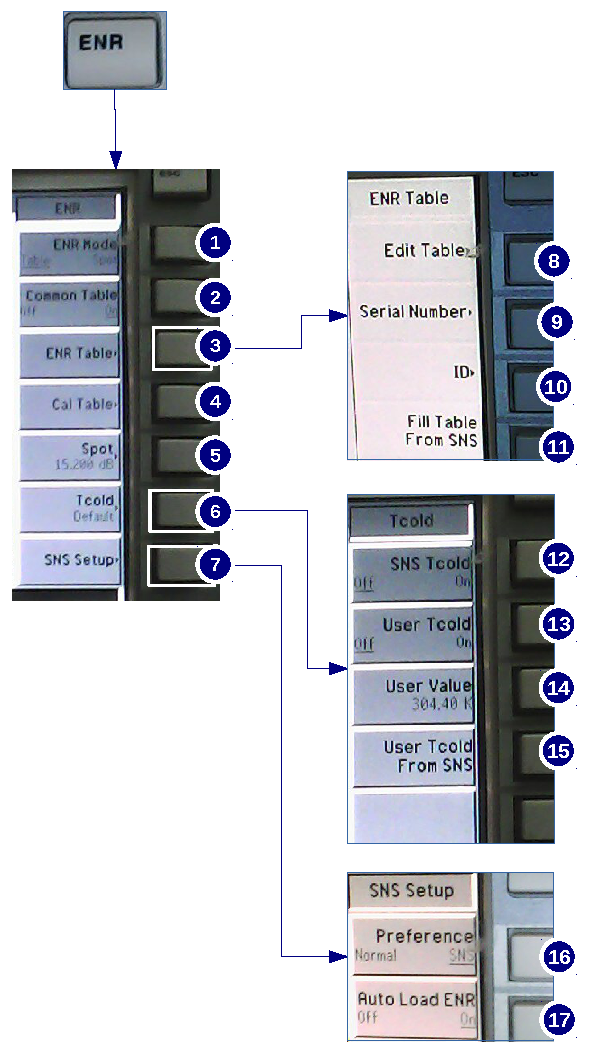
\includegraphics[width=0.5\textwidth]{./Imagenes/MenuENRN8975A.pdf}		
		\end{wrapfigure}
	
		\textbf{ENR}: permite introducir en el NFA \ todo lo relativo a los datos de la razón de excedente de ruido. Al presionar la tecla ENR del panel MEASURE se despliega en pantalla el menú de la figura 1. Se aprecia en la figura 1 que el NFA acepta los datos de ENR en formato tabular o en forma de valor
		puntual. El formato tabular le indica al equipo los valores de ENR para cada frecuencia de interés. En cambio se puede ingresar un único valor de ENR para ser utilizado en todo el rango de frecuencias de medición.	
		
		El equipo puede se configurado para aceptar dos tablas distintas de ENR al establecer la opción Common Table en Off. 
		
		El equipo puede aceptar dos tablas con datos de ENR, una de ellas se empleara exclusivamente en el durante el proceso de autocalibración (Cal Table) y la otra se usará para el proceso de medición ENR table.
		
		Cuando el modo de ENR esta establecido en Tabla, a través de las opciones y se pueden ingresar o editar las tablas de ENR para medición y calibración. Al presionar la tecla  espectiva, en pantalla se despliega el editor de tablas de ENR (figura). 	
		
		Cuando el modo ENR se configura en Spot, se ingresa un único valor de ENR con la opción de
		menú el cual se utilizara para todas las frecuencias de medición.
		
		A través del menú el usuario puede configurar el valor que empleará como temperatura física que posee la fuente de ruido, indicada en el menú como Tcold \ o temperatura fría. Al presionar esta opción, el usuario puede indicar si desea que el NFA cargue el valor de Tcold desde el sensor de temperatura de la fuente de ruido inteligente (SNS Tcold = On) o si debe tomar el valor establecido por el usuario (User Tcold = On). Cuando esta última opción esta activa, el usuario al presionar User Value y utilizando el teclado numérico puede ingresar el valor de Tcold o puede cargar el valor de Tcold desde la SNS
		
		El menu ENR permite establecer si el NFA empleará una fuente de ruido inteligente de la serie Agilent N4000 (SNS, serie N4000) o una fuente de ruido normal, serie 346 de Agilent. El NFA tiene la capacidad de cargar los datos de ENR de forma automatica cuando detecta	la conexión de una fuente de ruido SNS, con pción \ Auto Load ENR establecida en On.
	\end{minipage}
	
	\newpage		
	
	\begin{minipage}[t]{\textwidth}	
		\begin{wrapfigure}{r}{0.5\textwidth}	
			\centering	
			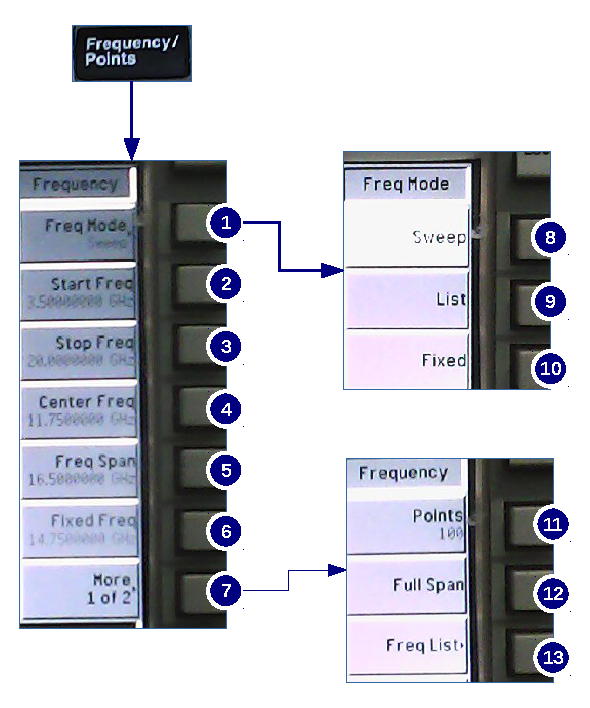
\includegraphics[width=0.5\textwidth]{Imagenes/MenuFrequencyPointsN8975A.pdf}	
		\end{wrapfigure}	
		
		\textbf{Frequency / Points} el NFA puede realizar mediciones sobre un rango de frecuencias, una lista de frecuencias oen una frecuencia puntual. Por medio de la opción Freq Mode se puede establecer que el NFA realize la medicion en forma	de barrido sobre un rango de frecuencias , sobre una lista de frecuencias, o en una frecuencia puntual (Fixed) 
		
		Cuando se utiliza el modo de barrido, el rango de frecuencias se especifica ya sea por su frecuencia de inicio y por su frecuencia final o bien por la frecuencia central del rango y su extensión. El numero de puntos \ que posee el rango se introduce con [Warning: Draw object ignored][Warning: Draw object ignored][Warning: Draw object ignored][Warning: Draw object ignored][Warning: Draw object ignored]Cuando se utiliza el modo de barrido, el rango de frecuencias se especifica ya sea por su frecuencia de inicio y por su frecuencia final o bien por la frecuencia central del rango y su extensión. El numero de puntos \ que posee el rango se introduce con 
				
		Cuando se establece el NFA que realice las mediciones sobre una lista de frecuencias, al presionar la
		opción, se muestra en pantalla el editor de lista de frecuencia sobre el cual el usuario ingresa los valores de frecuencia por medio del teclado numérico.][Warning: Draw object ignored][Warning: Draw object ignored]Cuando se establece el NFA que realice las mediciones sobre una lista de frecuencias, al presionar la opción, se muestra en pantalla el editor de lista de frecuencia sobre el cual el usuario ingresa los valores de frecuencia por medio del	teclado numérico.
		Cuando se desea medir en una frecuencia puntual, esta se ingresa por medio de la opción ][Warning: Drawobject ignored]Cuando se desea medir en una frecuencia puntual, esta se ingresa por medio de la opción. 		
	\end{minipage}
	
	\begin{minipage}[t]{\textwidth}
		\begin{wrapfigure}{l}{0.5\textwidth}	
			\centering	
			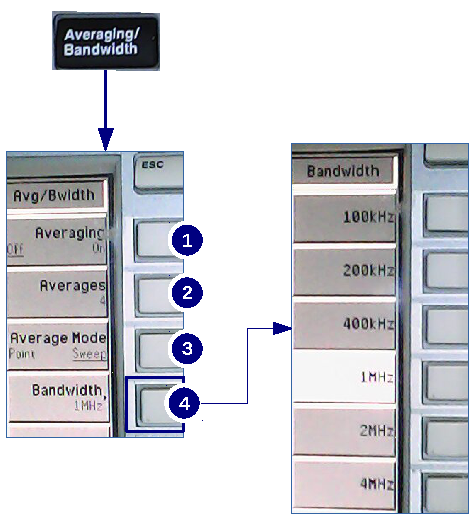
\includegraphics[width=0.5\textwidth]{Imagenes/MenuAverageBandwidthN8975A.pdf}	
		\end{wrapfigure}

		\textbf{Averaging / Bandwidth.} El promedio y el ancho de banda permite corregir los efectos del jitter del display en las mediciones. permite configurar el promedio y el ancho de banda. Para cada frecuencia de medición, el NFA mide la potencia de ruido en un ancho de banda centrado en torno a esta. El usuario puede elegir un valor para este ancho de banda de entre 6 opciones disponibles. El dispositivo puede ademas tomar múltiples mediciones y luego tomar el promedio de estas como el valor
		definitivo de la medición. Cuando se activa el promedio, el usuario puede especificar cuantas veces debe tomarse el mismo.	
		
		Al reducir el ancho de banda de medición, se incrementan los efectos del jitter en el display, lo cual puede corregirse incrementando el numero de promedios.
		
		Si se emplea un ancho de banda menor de 100 kHz, la cantidad de promedios debería ser 40 veces mayor si se desea obtener	la exactitud que se obtendría con un ancho de banda de 4 MHz.
		
		Si el promedio esta activo, el usuario puede seleccionar el modo de promedio (Average Mode) entre puntual (Point) \ o barrido (Sweep). Cuando se realiza el promedio puntual, el NFA calcula el promedio de	cada punto de frecuencia antes de avanzar al siguiente. Cuando el NFA ejecuta el promedio en barrido, el NFA realiza la	medición en un punto y avanza al siguiente. Cuando llega al ultimo punto, vuelve al primer punto toma una nueva medición y la promedia con el valor del último barrido, acumulando promedios en el tiempo. Esta opción permite ver el valor de la medicón en pantalla en tiempo real.
	\end{minipage}
	
	\begin{minipage}[t][11cm]{\textwidth}
		\begin{wrapfigure}{r}{0.5\textwidth}		
			\centering
			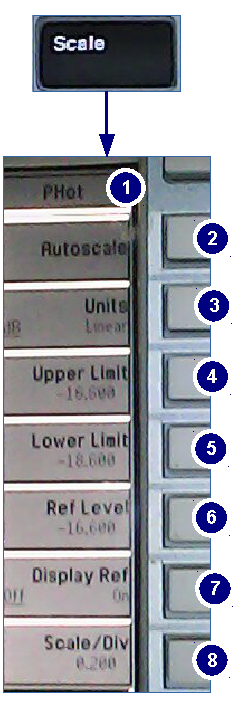
\includegraphics[height=10cm]{./Imagenes/MenuScaleN8975A.pdf}	
		\end{wrapfigure}
		
		\textbf{Scale.} Permite realizar ajustes relacionados a las escalas de los ejes en la presentación gráfica. La configuración de escala opera sobre el gráfico actualmente activo, se indica en el cual en la figura es un gráfico de PHot. Al presionar Autoscale la escala vertical de la gráfica activa se ajusta de modo automático para cubrir todo su rango de valores. Se puede seleccionar la unidad de presentación entre dB y lineal (Linear). \ Para la gráfica actualmente activa se puede ajustar los \ valores límites máximo y mínimo del eje vertical, así como también las unidades por división (Scale /
		Div).	
	\end{minipage}

	\begin{minipage}[t]{\textwidth}
		\begin{wrapfigure}{l}{0.5\textwidth}	
			\centering	
			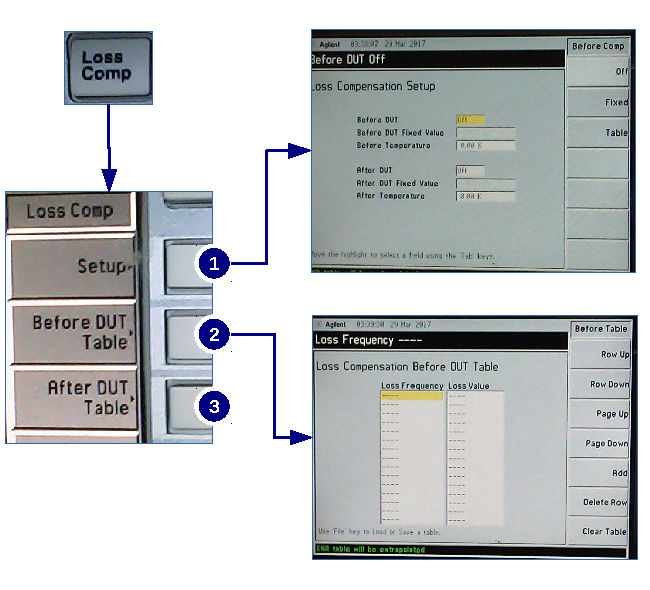
\includegraphics[width=0.5\textwidth]{Imagenes/MenuLossCompN8975A.pdf}	
		\end{wrapfigure}
		
		\textbf{Loss Comp.} permite realizar ajustes para compensar la atenuación y el ruido que	introducen los elementos presentes en el camino de señal, como cables y acopladores, ubicados antes y después del DUT. En la pantalla de edición se pude introducir un valor fijo de atenuación en los campos respectivos. También puede configurarse el equipo para aceptar o una tablas de valores de atenuación en función de la frecuencia en y luego ingresar las tablas de perdidas antes del DUT y después del DUT para las perdidas de los elementos antes y después del DUT. La pantalla cabia en este caso al modo de edición de tablas, donde se introduce un valor de frecuencia seguido de	su respectivo valor de perdidas.
		
		En se puede establecer la temperatura de ruido equivalente para los elementos antes o después del DUT. 
	\end{minipage}
	
	\begin{minipage}[t][10cm]{\textwidth}
		\begin{wrapfigure}{r}{0.5\textwidth}		
			\centering
			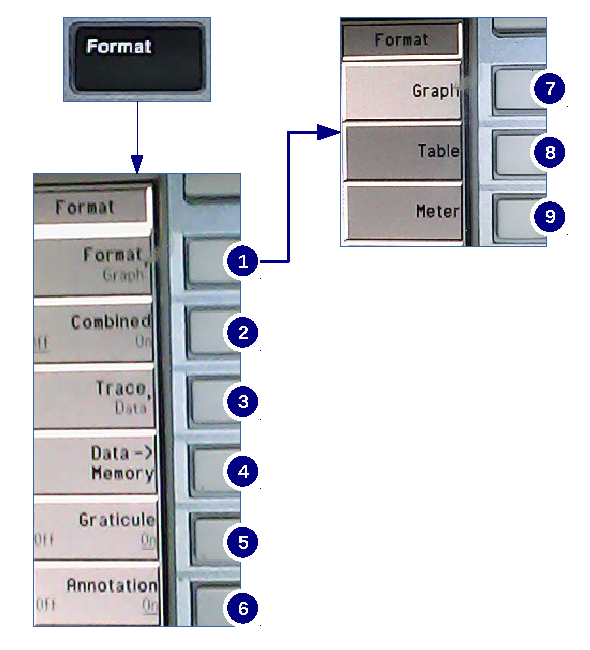
\includegraphics[width=0.5\textwidth, height=10cm, keepaspectratio]{./Imagenes/MenuFormatN8975A.pdf}	
		\end{wrapfigure}
		
		\textbf{Format.} Permite	seleccionar el formato de presentación de los datos de medición entre gráfico, tabla y valor puntual. Se \ puede activar la presentación de doble trazo en una única gráfica (Combined = On) o cada traza en su respectiva gráfica (Combined \ = Off), así como también activar la rejilla sobre los gráficos. 
		
		Pueden graficarse trazos almacenados en memoria del equipo, con y	
	\end{minipage}

	\begin{minipage}[t][10cm]{\textwidth}
		\begin{wrapfigure}{l}{0.5\textwidth}		
			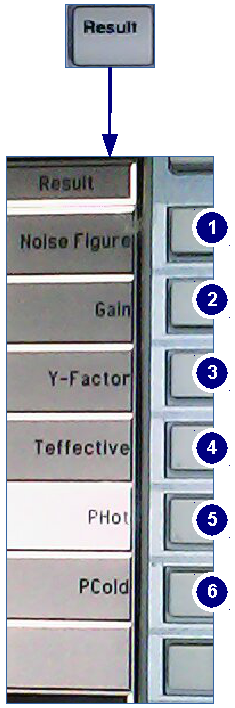
\includegraphics[width=0.5\textwidth, height=10cm, keepaspectratio]{./Imagenes/MenuResultN8975A.pdf}	
		\end{wrapfigure}
		
		\textbf{Result}: permite	elegir el valor de la medición que se visualiza en el gráfico activo, como la figura de ruido, la ganancia, el factor Y, la temperatura efectiva de ruido, la potencia de ruido “caliente” (fuente de ruido encendida) o la potencia de ruido fría.
	\end{minipage}



	%https://tex.stackexchange.com/questions/118602/how-to-text-wrap-an-image-in-latex
	%https://tex.stackexchange.com/questions/89821/how-to-draw-a-solid-colored-circle
	%https://tex.stackexchange.com/questions/96340/how-to-place-a-textnode-at-the-center-of-a-drawn-rectangle
	
	\begin{minipage}[t][11cm]{\textwidth}
		\begin{wrapfigure}{r}{0.5\textwidth}		
			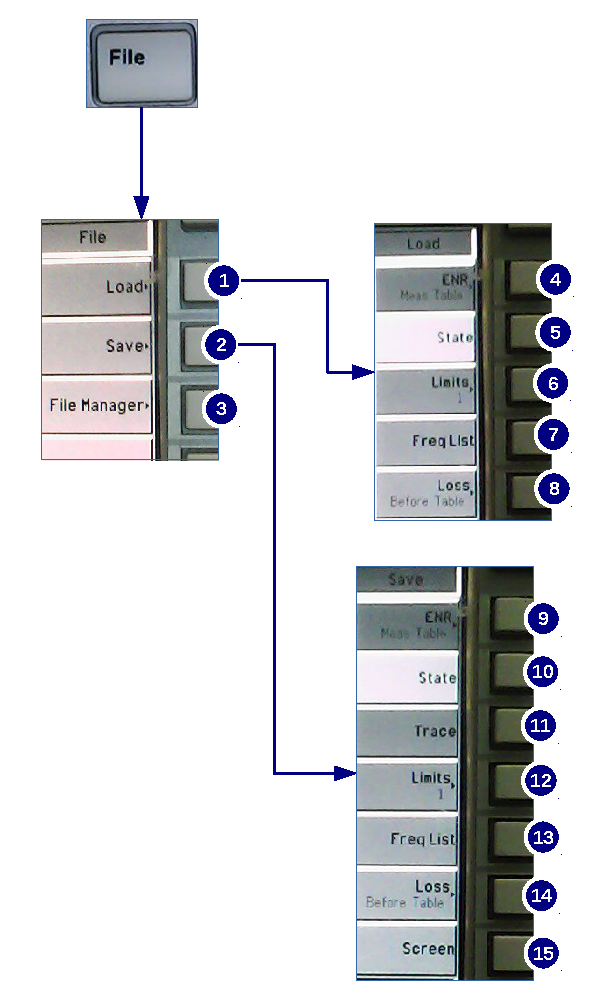
\includegraphics[width=0.5\textwidth, height=11cm, keepaspectratio]{./Imagenes/MenuFileN8975A.pdf}	
		\end{wrapfigure}		
		\textbf{File.} El N8975 posee la capacidad de almacenar información en su memoria interna o en un disco floppy, en forma de archivos. Al presionar la tecla File se presenta un menú con las funciones básicas sobre el sistema de archivos, Las opciones de menú permiten \ cargar (Load) y guardar (Save) archivos. La opción de menú , File Manager, presenta el administrador de archivos, por medio del cual se pueden copiar, renombrar y eliminar archivos, asi como también formatear un diskette en la unidad floppy.
		
		El N8975 puede almacenar o cargar archivos con tablas de ENR, estado del sistema, trazos limites, tablas de perdidas y gráficos desde o hacia la pantalla. 
	\end{minipage}


	\begin{minipage}[t][10cm]{\textwidth}
		\begin{wrapfigure}{l}{0.5\textwidth}		
			\centering
			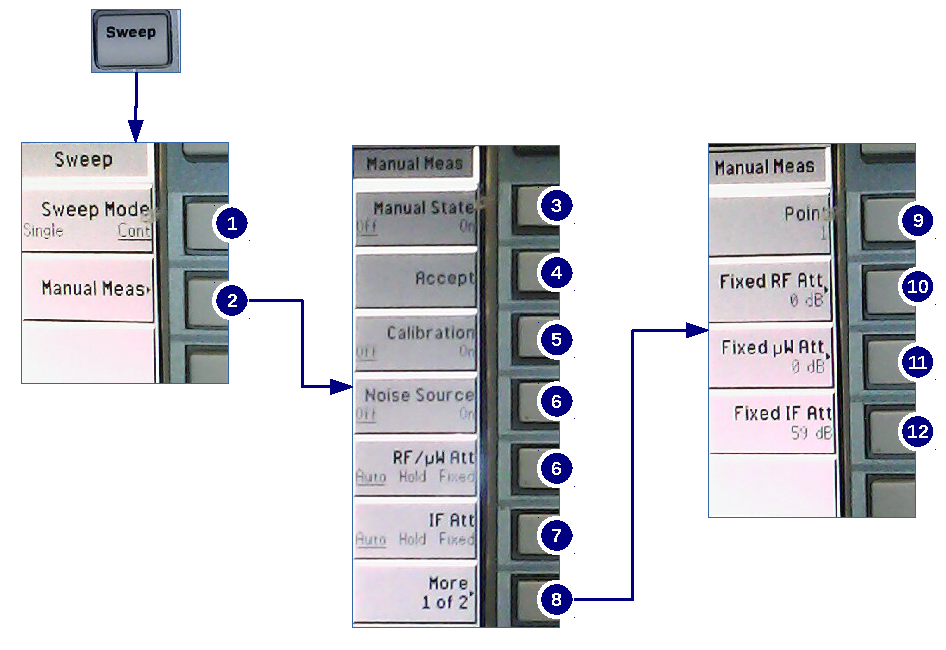
\includegraphics[width=0.5\textwidth]{./Imagenes/MenuSweepN8975A.pdf}	
		\end{wrapfigure}
		
		\textbf{Sweep.}		
	\end{minipage}
		
	Teclas de acción
	
	Al presionar se ejecuta un acción Calibrate, Full screen, Restart, Save Trace and Print.
	
	Capacidades del N8975
	
	Medición de potencia de ruido (PHOT, PCOLD~).
	
	Medición de Temperatura efectiva.
	
	Determinación del factor Y.
	
	Determinación de la figura de ruido.
	
	Medición de Ganancia.
	
	Puede ejecutar medidas en dispositivos simples o en sistemas de conversión de frecuencias.
	
	Mediciones básicas
	
	Preparación para proceso básico de medición
	
	Antes de realizar alguna medición de parámetros de ruido con el N8975, por lo general se deben ejecutar unos pasos
	previos de configuración del equipo.
	
	Para la medición de figura de ruido, el usuario debe ingresar ciertos datos al NFA antes de dar marcha con la medición.
	
	\begin{itemize}
		\item Ingresar los datos de la razón de ruido en exceso (ENR).
		\item Establecer el rango de frecuencias o la frecuencia individual sobre las cueles se desea la medida.
		\item Establecer el ancho de banda y configurar el promedio.
		\item Calibrar el analizador.
		\item Mostrar los resultados en pantalla.
	\end{itemize}

	Ingresar datos de ENR
	
	[Warning: Draw object ignored]El NFA requiere los datos de ENR de las fuentes de ruido que se utilicen durante las
	mediciones. El equipo emplea los valores de ENR en dos situaciones distintas: \ durante el proceso de auto-calibración
	y durante la medición de figura de ruido. Cuando el equipo ejecuta la auto-calibración, éste emplea una tabla de
	valores ENR de la fuente de ruido con la cual se lleva acaba este ajuste, por medio del cual el equipo elimina su
	contribución de ruido en la medición. Durante la medición de figura de ruido, el equipo emplea los datos de ENR de la
	fuente de ruido y mediciones directas de potencia de ruido para calcular y presentar en pantalla el valor F. 
	
	El N8975 admite el ingreso de los datos ENR se ingresan al N8975 en forma de tabla o en forma de valor puntual (spot
	value). \ Para el formato tabla, cada fila de esta consiste en un par de valores, frecuencia y ENR, esta tabla se
	emplea para medición en múltiples frecuencias. Si el equipo necesita el valor de ENR en alguna frecuencia que no este
	listado en esta tabla, simplemente calculará el valor que necesita por interpolación. \ Esto ocurre cuando la
	configuración establecida por el usuario para la frecuencia máxima, frecuencia \ mínima \ y cantidad de puntos de
	medición provocan que el rango de frecuencias sobre el cual medirá el NFA no concuerde con las frecuencias de la tabla
	ENR. 
	
	Debería medirse el DUT a las mismas frecuencias que establece la tabla de ENR de la fuente de ruido.
	
	Cuando se ingresa un valor puntual de ENR, el equipo lo emplea para medición en una sola frecuencia \ es aplicado en
	todo todo el rango de medición.
	
	El equipo puede operar con \ dos tablas distintas para ENR: una tabla para ENR de calibración \ y una tabla para valores
	de ENR de medición. La tabla ENR de calibración la emplea el equipo cuando ejecuta el proceso de auto-calibración. La
	tabla ENR de medición la emplea el equipo \ durante la medición de figura de ruido. \ 
	
	Puede configurarse el equipo para que utilice dos tablas de ENR distintas (calibración y medición) o para que utiliza
	una única tabla de ENR, la tabla ENR de calibración, para la tarea de auto calibración y medición de figura de ruido.
	
	La utilidad en emplear dos tablas de ENR esta en que se puede emplear una fuente de ruido para el proceso de
	auto-calibración y otra fuente de ruido distinta para el proceso de medición. 
	
	La fuentes de ruido normales, como las \ Agilent 346, el usuario debe ingresar \ de forma manual o por medio de un
	diskette que le suministra el fabricante los datos de ENR, el fabricante suministra estos datos. La fuentes de ruido
	inteligentes de Agilent (SNS) pueden cargar los datos de ENR de manera automática al NFA.
	
	Los puntos de frecuencia a medir son determinados por entradas en la tabla de ENR?
	
	Los datos de ENR pueden cargarse de cuatro formas distintas maneras:
	
	\begin{itemize}
		\item Se puede ingresar un único valor de THOT
		\item Puede introducir datos de ENR por medio de un disco floppy, en donde previamente se haya almacenado la data de
		Introduciéndolo en la ranura que dispone el NFA y utilizando el administrador de archivos. Se accede a las funciones e
		control de archivos por medio del botón File (panel System).
		\item Puede cargar los datos desde la memoria interna del NFA. 
		\item Puede cargar los datos de forma remota, a través del bus GPIB. 
		\item En caso de utilizar una fuente de ruido inteligente, como las Agilent serie N4000, el usuario puede elegir si
		cargar de foma automática cuando se conecte una fuente de ruido.
	\end{itemize}
	Ingresar datos de temperatura (TCOLD)
	
	En caso de que la temperatura en el recinto donde se efectúe la medición sea distinta a la temperatura por defecto
	establecida en el equipo de 296.05K, se debe ingresar al equipo el valor de la temperatura (TCOLD). Cuando se emplean
	las fuentes de ruido inteligentes SNS, serie Agilent N4000, este paso puede \ ya que estas fuentes incluyen un sensor
	de temperatura interno, el NFA puede cargar automaticamente el valor de temperatura correcto al momento de efectuar
	cada medición.
	
	Establecer las frecuencias de medición
	
	El usuario debe establecer el conjunto de frecuencias sobre las cuales se realizará la medida. El N8975 dispone de tres
	opciones para la selección de frecuencias de medición: barrido (swep), lista (list) y fija (fixed).
	
	Barrido (sweep): el rango de frecuencias de medición se obtiene de una frecuencia inicial, una frecuencia final y el
	numero de medidas.
	
	Lista (list): las frecuencias de medición se especifican ingresando en el N8975 una lista de valores de frecuencia.
	
	Fija (fixed): el usuario establece que la medición se realizará en un único valor de frecuencia.
	
	Establecer el ancho de banda y activación del promedio.
	
	Se selecciona un valor para el \ ancho de banda, el cual determina \ en torno a cada valor de frecuencia sobre el cual
	se integra la potencia de ruido. El usuario debe escogen un valor de ancho de una lista, las opciones para el ancho de
	banda son \ 100 kHz, 200 kHz, 400 kHz, 1 MHz, 2Hz y 4MHz.
	
	El usuario puede elegir si desea activar el promedio en las mediciones. Si se activa el proedio, puede establecer si es
	un promedio puntual o promedio de barrido.
	
	Al activar el promedio el jitter y se provee de mediciones más precisas cuanto más promedios se realice. Sin embargo, la
	velocidad de medición se reduce.
	
	Calibración
	
	Cumplidos los pasos anteriores, se ejecuta la auto calibración del equipo N8975. La auto calibración le permite a este
	equipo compensar la contribución de ruido introducida por el cableado y accesorios que se encuentren en el camino de
	señal además del ruido generado por el propio N8975.		
	
	\begin{figure}
		\centering
		\begin{minipage}{8.063cm}
			%\includegraphics{Imagenes/EsquemaConexionCalibracion.png}
			\caption{Conexión del sistema para ejecutar auto calibración.}
		\end{minipage}
	\end{figure}
	Se conecta el equipo con indica la figura. Los datos de ENR para la fuente de ruido empleada en la calibración deben haberse introducido previamente en la tabla de calibración.
			
	Mostrar resultados
	
	El equipo puede presenta los resultados en forma de gráficos, tabla o valor textual. En cuanto a la presentación de	gráficos, el equipo puede presentar dos resultados en pantalla de manera simultanea o combinarlos en un mismo gráfico. Puede salvar la gráfica activa en memoria.
	
	Interruptor mecánico de 3GHz
	
	El NFA N8975 posee un interruptor mecánico ajustado para conmutar del rango de frecuencia de 10 MHz a 3.0 GHz al rango	de 3.0GHz a 26.5GHz. Si el rango de frecuencia que seleccione el usuario cruza el punto de 3.0GHz, el switch mecánico se activa. El interruptor mecánico tiene un un numero limitado de activaciones sobre el cual es confiable. La	conmutación sobre los 3.0 GHz debe limitarse siempre que sea posible
	
	Antes de emplear el N2002A debe realizarse un test de verificación, para asegurar que los caminos de conmutación	funcionen y que el VSWR este dentro de los limites [1.19]	
	
	%\subsection{Banco de atenuadores y aisladores N2002A (Noise Source Test Set )}
El banco de atenuadores y aisladores N2002A (figura \ref{Fig:BancoAtenuadoresAisladores}) es un dispositivo que, de acuerdo a la nota de aplicación de Agilent Technologies \cite{AGI02}, esta destinado a facilitar la calibración de fuentes de ruido de forma rápida y precisa. Es un instrumento que se integra a un sistema para calibración de fuentes de ruido, como el mostrado en la figura \ref{Fig:BancoPruebasFuenteRuido}. 		

\begin{figure}[h!]
	\centering
	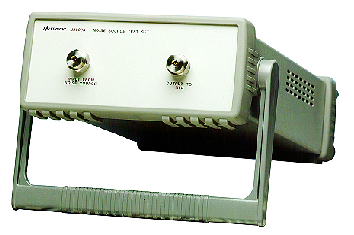
\includegraphics[height=6cm]{./Imagenes/BancoAtenuadoresAisladoresN2002.pdf}
	\caption{Interfaces eléctricas del N2002A}			
	\label{Fig:BancoAtenuadoresAisladoresN2002.pdf}
\end{figure}

En la medición de figura de ruido de alta precisión la incertidumbre de esta esta fuertemente relacionada a la incertidumbre de la fuente de ruido empleada en la medición. Al conformar un banco de calibración de NS empleando el N2002A, se pueden realizar mediciones de alta precisión en “casa”, lo que evita recurrir a laboratorios especializados	para efectuar esta tarea.

se debe emplear cuando se efectúan mediciones de ENR alta precisión en fuentes de ruido.

El N2002A se inserta en el camino de señal de RF o UW, entre la salida de la fuente de ruido bajo prueba y la entrada	del NFA. La función de este es de proveer aislamiento entre la fuente de ruido y el NFA con el fin de minimizar el	coeficiente de reflexión. Las reflexiones entre el DUT y la fuente de ruido causan incertidumbre en la potencia de ruido que emerge de la fuente; la medición entonces no se refiere a la impedancia de 50 Ohms deseados, sino a la impedancia actual de la fuente de ruido. Incorporando el N2002A dentro del sistema de calibración se minimiza la interacción entre el DUT y el NFA, minimizando el coeficiente de reflexión y de esta forma la incertidumbre. Esto
permite una calibración más precisa de la fuente de ruido, asegurando precisión, repetibilidad y trazabilidad en las	mediciones ademas de reducir de manera significativa la incertidumbre [2].	

En la figura \ref{Fig:VistaInternaN2002} se muestra una vista interna y en la figura \ref{Fig:EstructuraInternaN2002} una vista esquemática de la estructura interna del dispositivo. Se aprecia que este equipo esta conformado por cuatro secciones de atenuadores y una sección de aislador. Los atenuadores o el aislador son conectados o desconectados del camino de señal por medio dos conjuntos de interruptores, etiquetados como A2 y A6 respectivamente en la figura 3. Las señales que controlan estos interruptores provienen del exterior del equipo, son generadas por un dispositivo de la serie 11713 de Agilent / Keysight Technologies, unidad controladora de atenuadores e interruptores. Cada sección de atenuador permite el paso de señal en un rango de frecuencia distinto,
como se indica en la figura 3. El N2002A cubre un rango de frecuencias idéntico al del N8975, va desde \SI{10}{\mega\hertz} MHz hasta \SI{26.5}{\giga\hertz}. 

\begin{figure}[h!]			
	\centering
	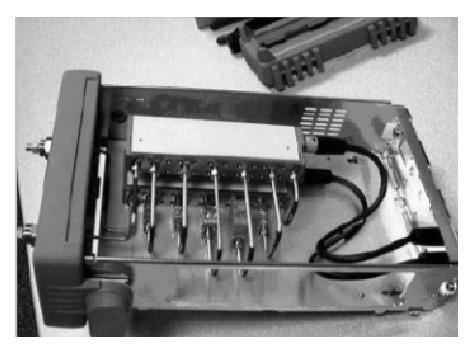
\includegraphics[width=15cm]{Imagenes/VistaInternaN2002.pdf}
	\caption{Esquema de la estructura interna para el N2002S}
	\label{Fig:VistaInternaN2002}
\end{figure}

El N2002A no posee fuente de poder interna ni tampoco realiza mediciones. No dispone de interfaz de usuario, este equipo debe ser comandado por medio de un dispositivo de la serie 11713. EL 11713 brinda la interfaz de usuario necesaria, en	éste el usuario realiza la selección del rango de frecuencia sobre el cual N2002A debe permitir el paso.		

El N2002A cuenta únicamente con interfaces eléctricas dispuestas en el panel frontal y posterior del equipo (figura \ref{Fig:InterfacesElectricasN2002}). La interfaz para señal de RF / UW esta dispuesta en el panel frontal (figura	\ref{Fig:InterfacesElectricasN2002}a) y posee dos conectores, un conector es la entrada de señal en el cual se conecta la fuente de	ruido (izquierda) y el otro conector es la salida filtrada o atenuada la cual se conecta a la entrada de señal del NFA (derecha). En en el panel posterior se encuentra la interfaz para señales de control (figura \ref{Fig:InterfacesElectricasN2002}b), en esta se encuentran dos conectores para las señales generadas por un dispositivo de la serie 11713.		

\begin{figure}[h!]
	\centering
	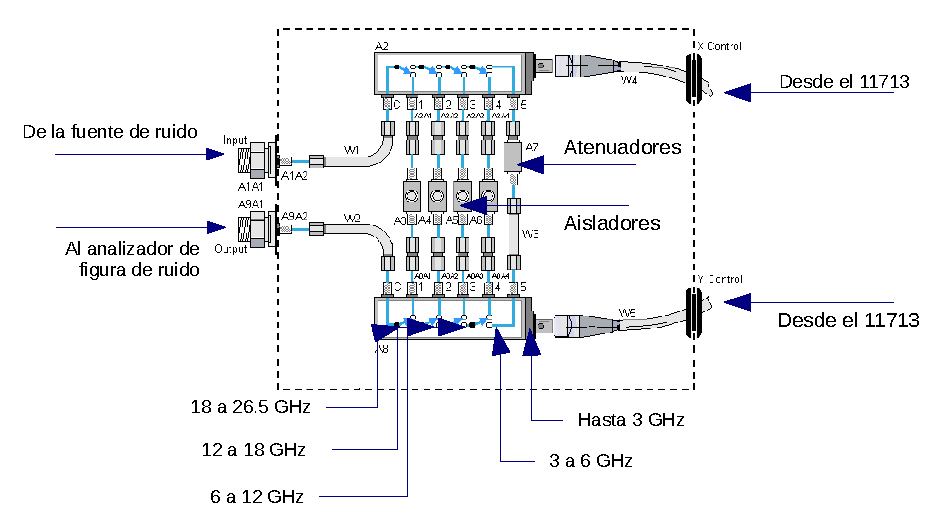
\includegraphics[width=15cm]{Imagenes/EsquemaEstructuraInternaN2002.pdf}
	\caption{Esquema de la estructura interna del N2002A}			
	\label{Fig:EsquemaEstructuraInternaN2002}
\end{figure}

\begin{table}[h!]
	\centering
	\begin{tabular}{cccc}
		\toprule
		A1 & Aislador 18 \si{\giga\hertz} – 26,5 \si{\giga\hertz} \\
		\midrule
		A2 & Aislador 12 \si{\giga\hertz} – 18 \si{\giga\hertz} \\
		\midrule
		A3 & Aislador 6 \si{\giga\hertz} – 12 \si{\giga\hertz} \\
		\midrule
		A4 & Aislador 3 \si{\giga\hertz} – 6 \si{\giga\hertz} \\		
		\midrule
		A5 & Atenuador 3 \si{\decibel} \\				
		\bottomrule
	\end{tabular}
	\caption{Rangos de ENR nominal para fuentes de ruido serie N4000}
	\label{Tab:RangosFuentesRuido}
\end{table}

\begin{figure}[h!]
	\centering
	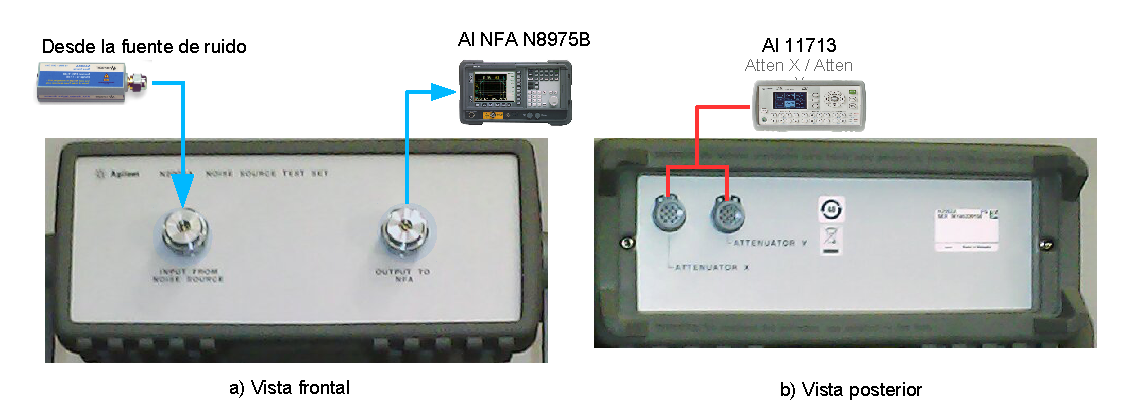
\includegraphics[width=16cm]{Imagenes/InterfacesElectricasN2002.pdf}
	\caption{Esquema de la estructura interna del N2002A}			
	\label{Fig:InterfacesElectricasN2002}
\end{figure}

Según recomendación de Agilent, se debe usar el N2002A en conjunto con el Agilent N8975A (NFA) como equipo básico fundamental para calibración de fuente de ruido. N2002A es un equipo para calibrar fuentes de ruido “en casa” [3.3]. El objetivo es calibrar fuentes de ruido a estándar trazables.

Permite calibrar de manera rápida, repetible con niveles mínimos de incertidumbre. Este equipo es necesario cuando se	realizan pruebas de ENR sobre una fuente de ruido. Asegura resultados de calibración precisos, incrementa la confianza en la medición, permite el desarrollo de DUTs con especificaciones más exigentes. Entrega resultados trazables a 	estándares nacionales.

\begin{figure}
	\centering
	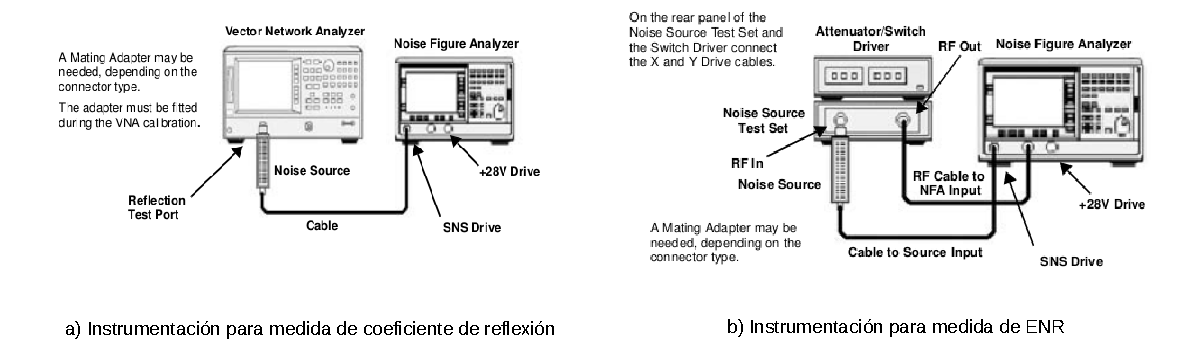
\includegraphics[width=5cm]{Imagenes/InstrumentacionCalibracionN2002.pdf}
	\caption{Instrumentación para calibración de fuentes de ruido}
	\label{Fig:InstrumentacionCalibracionN2002}
\end{figure}

El proceso de calibración consiste en comparar el desempeño de forma trazable de una fuente de ruido en relación al desempeño de otra fuente de ruido, que se toma como estándar de calibración, o contra las especificaciones del fabricante. Para ello se realizan \ dos pruebas de verificación de desempeño: 

\begin{itemize}
\item Medición de la razón de ruido excedente (ENR).
\item Medición del coeficiente de reflexión complejo (magnitud y fase). 
\end{itemize}

Si la fuente de ruido falla cualquiera de estas pruebas es indicador que requiere reparación o ajuste.

El sistema de calibración de Agilent permite verificas las fuentes de ruido Agilent de la serie 346 (346A, 346B, 346C) y las fuentes de ruido inteligentes de la serie Agilent N4000A (N4000A, N4001A, N4002A). Este proceso de calibración permite calibrar fuentes de ruido entre \SI{10.0}{\mega\hertz} y \SI{26.5}{\mega\hertz}. 

En la figura \ref{Fig:InstrumentacionCalibracion} se muestra la instrumentación propuesta por Agilent \cite{AGI03} para la medida de coeficiente de reflexión (figura \ref{Fig:InstrumentacionCalibracion}a) y para la medida del ENR (figura \ref{Fig:InstrumentacionCalibracion}b).	

\begin{table}
	\centering
	\begin{tabular}{m{6cm}m{6cm}}
		\toprule
		\textbf{Coeficiente de reflexión} 	&	\textbf{ENR}	\\
		\midrule
		Analizador de red que cubra el rango 10 \si{\mega\hertz} a 26.5 \si{\giga\hertz} (VNA) 8753ES o 8753ET, 8722ES o 8722ET 	&	Analizador de figura de ruido N8975A \\
		\midrule
		Analizador de figura de ruido N8975A	&	N2002A conjunto para pruebas con fuentes de ruido \\
		\midrule		
		Kit de calibración para VNA			&	Controlador de atenuadores e interruptores 11713 \\
		\midrule		
		Controlador de atenuadores e interruptores 11713	& 	Fuente de ruido referencia estandar \\
		\midrule		
		Cable Viking para conexión del 11713	&	\\
		\bottomrule		
	\end{tabular}
\end{table}

\subsection{Descripción de las pruebas de verificación}
\subsubsection{Medición de ENR}
La prueba de ENR consiste en comparar los resultados de la prueba sobre una fuente de ruido bajo prueba (DUT) contra los	resultados de una prueba sobre una fuente de ruido referencia estándar. La referencia estándar es una fuente de ruido calibrada con valores conocidos de ENR. Las medidas se llevan a cabo tanto en la fuente de ruido DUT asi como en la fuente de ruido referencia estándar. Los valores de ENR del DUT se derivan de estos resultados. 

Los resultados de esta prueba permiten asegurar si la fuente de ruido cumple con las especificaciones de calibración del fabricante. La precisión de la medidas para el DUT es altamente dependiente de la exactitud de la calibración de la referencia estándar. Se debe usar, según Agilent, una referencia estándar que haya sido calibrada por un laboratorio especializado.

Las pruebas deben realizarse dentro de la temperatura ambiente de 296 ± 1K (23 ± 1) °C.

Las fuentes de ruido requieren calibración periódica del desempeño operacional. En condiciones de uso normal y ambientales, se calibra la NS cada 12 meses [1.27].

\subsubsection{Resumen del procedimiento de medición de ENR [1.29] [1.39].}
Se emplea la instrumentación indicada en la figura \ref{seq:refDrawing4}b. Se inicia el proceso al encender los equipos y permitir que calienten por una hora. Se debe permitir que las fuentes de ruido se estabilicen a la temperatura	ambiente. No se deben usar las fuentes de ruido una hora antes de realizar las mediciones.
	
Se deben cargar los datos de ENR de la fuente de ruido referencia estándar en el analizador de figura de ruido. Estos datos los proporciona el fabricante de la NS ya sea en formato digital o físico. SI se usa una fuente de ruido inteligente (SNS), el NFA puede cargar los datos de ENR que se encuentran en la memoria de la SNS de forma automática, si el NFA esta habilitado.

La secuencia de pasos para la medición emplea las tabla \ref{seq:refDrawing5}a para registro de resultados

\begin{itemize}
\item Los valores de ENR de la referencia estándar (ENR1) son conocidos, ingresar estos valores en la columna ENR1 de la
tabla 1.
\item Se conecta el equipo de prueba como indica la figura \ref{seq:refDrawing4}b.. Conectar la fuente de ruido de
referencia, asegurando que el conector RF de esta NS es del mismo tipo que el conector de la NS DUT]. Ajustar los
interruptores del 11713, para el canal de frecuencia requerido, por ejemplo interruptores 9 y 0 ON para medir entre
10MHz y 3.0GHz. 
\item Establecer el equipo para realizar la medida del primer punto de frecuencia. 
\item Medir el factor Y lineal de la NS referencia estándar.
\item Anotar este valor en la tabla , bajo la columna Y1.
\item Establecer el equipo para medir el siguiente punto de frecuencia, repetir el procedimiento hasta que todos los
puntos de medición estén completos.
\item Remover la referencia estándar de la entrada del N2002A y la NS DUT.
\item Establecer el equipo para medir el primer punto de frecuencia.
\item Medir el factor Y lineal en la NS DUT.
\item Anotar en las tablas de registro el resultado bajo la columna Y2.
\item Repetir el procedimiento para todos los puntos a medir.
\item Con los resultados obtenidos, introducirlos en las ecuaciones y calcular con ellas el ENR y los valores de
incertidumbre.
\end{itemize}

Conectar cables Viking de la parte posterior del 11713A a la parte posterior del N2002A. Conectar Atten X del 11713A al Attenuator X del N2002A. Conectar Atten Y del 11713A al Attenuator Y del N2002A.

Proceso de Calibración [1.26]	
SI la fuente de ruido falla cualquiera de estas pruebas de desempeño, la NS requiere reparación.

Aparte de la calibración en puntos cardinales de frecuencia, se puede realizar la calibración en otros puntos. El máximo de puntos frecuencia-ENR es de 81.
	
Tabla de VSWR típico en [1.19]

Agilent N2002A empleado cuando se requiere realizar pruebas de Razón de Ruido en Exceso (ENR) sobre una fuente de ruido [1.14]. 

\subsubsection{Ecuaciones}
\emph{ENR}
\begin{equation}
	ENR_2 = 10\log\left(\frac{\left(Y_2-1\right)\left(T_0\frac{10^\frac{ENR_1}{10}}{Y_1-1}\right)}{T_0}\right)
\end{equation}

\emph{Incertidumbre}
\begin{equation}
	U_{C}ENR_2=\sqrt{(U_{C}ENR_1)^2+(U_{C}Sys)^2}
\end{equation}

donde

TO = 290 K.

ENR1 = Valor de ENR de la fuente de ruido de referencia en cada punto de frecuencia.

ENR2 = Valor calculado de ENR de la fuente de ruido DUT en cada punto de frecuencia.

Y1 = Valor medido del factor Y de la fuente de ruido de referencia en cada punto de frecuencia.

Y2 = Valor medido del factor Y de la fuente de ruido DUT en cada punto de frecuencia.

UcENR1 = Valor de incertidumbre de ENR de la fuente de ruido de referencia en cada punto de frecuencia.

UcENR2 = Valor calculador para la incertidumbre de ENR de la fuente de ruido de referencia en cada punto de frecuencia.

UcSys = Incertidumbre total del sistema de medición en cada punto de frecuencia.

	
\begin{figure}[h!]
\centering
 Tablas para registro
	de datos, relativos a la medición de ENR
\end{figure}

El N2002A es controlado por el 11713A. El 11713A es controlado por el software N2002A Noise Source Demonstration Software (No encontrado. Ver en su lugar VEE PRO en KeySight).

Equipo de Prueba Recomendado

Para mediciones de ENR y el coeficiente de reflexión (magnitud \ y fase), equipo listado en las tablas 2-4 y 2-5 del
documento [1].		

\subsection{Medición de coeficiente de reflexión (magnitud y fase) [1.31]}
\subsection{Rango de las mediciones de ENR para fuentes de ruido Agilent}
La medición de ENR sobre la fuente de ruido permite garantizar que esta se encuentre dentro de las especificaciones, por ejemplo dadas por Agilent en la tabla 1.		

Automatización del proceso de medición

El software que automatiza el proceso de medición esta escrito dentro de Agilent VEE Pro, el cual parece ser un entorno de ejecución (run time), esta disponible como un archivo VEE Pro o un archivo VEE Pro run time (posiblemente sea un script). 

\begin{itemize}
\item Software listado en [3.8]
\item Agilent VEE Pro
\item Agilent VEE Pro run time (provisto con el N2002A)
\end{itemize}
VEE Pro puede comunicarse a través de GPIB, LAN, USB, RS-232, VXI y LXI.

Para su uso requiere una tarjeta de interfaz GPIB (Agilent o National Instruments).

Sistema de calibración de fuente de ruido Agilent		

El sistema de la figura 1 cuenta con los equipos [2.5]:

\begin{itemize}
\item NFA N8975, opera en un rango de 10MHz a 26.6GHz) (con opción 1D5 la cual es una referencia de frecuencia de alta
estabilidad). 
\item Cuenta con el N2002A conjunto para pruebas con fuente de ruido que puede incluir todos los cables y conectores
necesarios para ejecutar calibración de NS con conectores de 3.5mm y tipo N (opción 001). Incluye el 11713A. 
\item Incluye una fuente de ruido estándar de oro.
\end{itemize}
Características del sistema [2.5]

Entre otras, puede calibrar fuentes de ruido tipo SNS y de la serie 346 de Agilent.

Nota importante de [2.3]

El N2002A conjunto para pruebas con fuente de ruido debe ser usado en un sistema de calibración de fuente de ruido, este
equipo no posee fuente de poder y no realiza mediciones.

\subsection{Equipo complementario al N2002A}
Según [2.4] este equipo cuenta con las fuentes de ruido inteligentes (SNS) Agilent de la serie N4000 y de la serie 346.

\subsection{Prueba de verificación [1.17]}
Por medio de un analizador vectorial de red se verifica el coeficiente sea el que indica la tabla para cada frecuencia.

\begin{table} 
	\begin{tabular}{ccc}
		\toprule
		\textbf{Frecuencia(\si{\giga\hertz})} & \textbf{Límite ROE \newline típico} & \textbf{Combinación \newline de botones 11713} \\
		\midrule
		0.01 	&	1:1.05	&	0 On, 9 On \\
		0.1 	&	1:1.05	&	0 On, 9 On \\
		1	 	&	1:1.05	&	0 On, 9 On \\
		2 		&	1:1.05	&	0 On, 9 On \\
		3 		&	1:1.05	&	0 On, 9 On \\
		4 		&	1:1.1	&	1 On, 5 On \\
		5 		&	1:1.1	&	1 On, 5 On \\
		6	  	&	1:1.1	&	1 On, 5 On \\
		7	 	&	1:1.15	&	3 On, 7 On \\
		8	 	&	1:1.15	&	3 On, 7 On \\
		9	 	&	1:1.15	&	3 On, 7 On \\
		10	 	&	1:1.15	&	3 On, 7 On \\
		11	 	&	1:1.15	&	3 On, 7 On \\
		12	 	&	1:1.15	&	2 On, 6 On \\
		13	 	&	1:1.15	&	2 On, 6 On \\
		14	 	&	1:1.15	&	2 On, 6 On \\
		15	 	&	1:1.15	&	2 On, 6 On \\
		16	 	&	1:1.15	&	2 On, 6 On \\
		17	 	&	1:1.15	&	2 On, 6 On \\																																				
		18	 	&	1:1.15	&	2 On, 6 On \\
		19	 	&	1:1.18	&	4 On, 8 On \\
		20	 	&	1:1.18	&	4 On, 8 On \\
		21	 	&	1:1.18	&	4 On, 8 On \\
		22	 	&	1:1.18	&	4 On, 8 On \\
		23	 	&	1:1.18	&	4 On, 8 On \\								
		24	 	&	1:1.15	&	4 On, 8 On \\
		25	 	&	1:1.18	&	4 On, 8 On \\
		26	 	&	1:1.18	&	4 On, 8 On \\
		26.5 	&	1:1.18	&	4 On, 8 On \\	
		\bottomrule	
	\end{tabular}
\end{table}





	%\subsection{Puente LAN/GPIB para Windows E5810}

El E5810 actúa como un puente entre una red LAN y equipos que soporten conexión GPIB y/o RS-232.  Permite   realizar operaciones I/O para obtener mediciones de datos de manera local o remota desde la instrumentación GPIB o RS-232.

\begin{figure} 
	\centering
	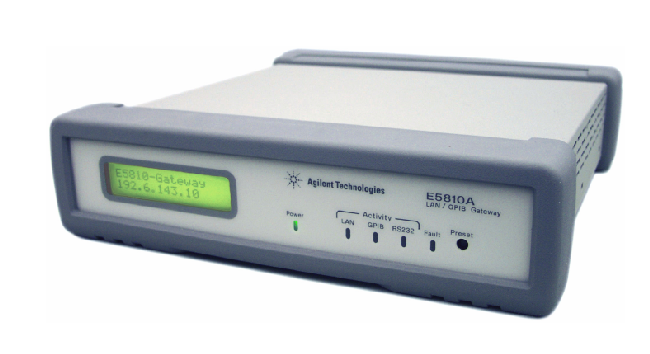
\includegraphics{Imagenes/E5810.pdf}
	\caption{Puente LAN/GPIB Agilent E5810}
	\label{Fig:PuenteLanGPIB}
\end{figure}

\subsubsection{Interfaz de comunicaciones}
Conexiones de red

EL E5810 puede conectarse a una red de la dos siguientes formas: 

\begin{itemize}
	\item Conexión a una red empresarial.
	\item Conexión a una red local.
	\item Conexión directa a una PC.
\end{itemize}

El E5810 puede servir de puente para 14 instrumentos GPIB y para un (1) instrumento RS-232, vía red Ethernet  10BASE-T/100BASE-TX. El E5810 puede detectar la configuración de red y ajustarse de forma automática a la velocidad apropiada. Este equipo posee un conector RJ-45 en su parte posterior. 

\subsubsection{Software}

El E5810 incluye \emph{Agilent IO libraries Suite}, la cual incluye Agilent Virtual Instrument Software Architecture (VISA), VISA COM, Standard Control Library (SICL) y varias utilidades I/O. Este software provee compatibilidad con diferentes fabricantes de software y hardware. Provee una capa de software para operaciones I/O, permite utilizar varios lenguajes como Visual Basic, Visual C++ y Agilent VEE.
El E5810 soporta Dynamic Host Configuration Protocol (DCHP el cual le permite obtener su dirección de IP de forma automática. Por defecto el equipo puede usar DHCP, se puede deshabilitar DHCP y asignar una dirección estática IP al E5810.
El E5810 soporta todas operaciones I/O provistas por VISA, VISA COM, SICL y Agilent VEE. 
Como se muestra en la figura 1, el PC posee las aplicaciones cliente VISA LAN, TCP/IP LAN, necesarias para acceder al E5810. El E5810 posee un servidor LAN además de firmware TCP/IP LAN que le permite actuar como un servidor LAN.
El software cliente realiza conexión con el servidor remoto dentro del E5810, establecida la conexión, el cliente envía peticiones I/O al servidor E5810 a través de la red al servidor E5810, el software instalado en la PC cliente VISA LAN emplea la suite de protocolos TCP/IP LAN para ello. El servidor del E5810 ejecuta estas peticiones de I/O en el instrumento GPIB o RS-232 apropiado.
El E5810 pude servir a múltiples clientes conectados en un momento dado. La cantidad máxima de clientes concurrentes depende del uso de memoria de E5810, la cual esta determinada por el numero de clientes y el numero de sesiones que corren estos clientes. Existe un máximo de 16 clientes accediendo de forma concurrente.
Múltiples instrumentos GPIB se pueden conectar al bus GPIB, pero solo una operación de I/O puede ocurrir en el bus GPIB en un momento dado. Solo se ejecuta una petición de un cliente a la vez, las demás deben esperar hasta que el cliente actual termine. El primer cliente en acceder es el primer cliente servido (cola FIFO).
En caso de que el cliente requiera realizar una secuencia de operaciones I/O que no deban ser interrumpidas, el cliente debe obtener un lock sobre la interfaz GPIB del dispositivo. Completada la operación debe liberar el lock.






	\subsection{Conectores}
El rango de frecuencia de cualquier conector esta limitado por el primer modo de propagación de la guía de onda circular en la estructura coaxial. Disminuir el diámetro del conductor externo incrementa la más alta frecuencia usable. Rellenar el espacio de aire con dieléctrico disminuye la frecuencia más alta usable.

Si las dimensiones mecánicas de los conectores no esta apareada, si el enchapado/plating no es el adecuado, o si la separación de contactos en la unión es excesiva, el coeficiente de reflexión y las perdidas resistivas se incrementan.

\subsubsection{Conector tipo N}
Conectores de propósito general, sexuados, relativamente económicos. Conectores robustos de 7 mm se desempeña bien en entornos de operación extremos y en aplicaciones que requieran conexiones repetidas.

El conector tipo N (Navy) de 50 Ohm fuen diseñado en la decada de 1940 para uso militar, operando inicialmente a 4 GHz. Posteriormente en la decada de 1960 lo avances tecnologicos incrementaro la frecuencia a 12 GHz y luego, en modo libre, hasta 18 GHz.

\subsubsection{Conector 3.5mm}

Conectores de precisión de 3.5 mm, sexuados con dieléctrico de aire. El aire provee aislamiento dieléctrico entre el conductor central y externo. Una arandela plástica dentro del cuerpo del conector soporta al conductor central.
Los conectores de 3.5 mm hacen juego con conectores SMA. Los conectores de 3.5 mm son lo suficientemente duraderos pra uso en repetidas conexiones.
El conector de 3.5 mm fue desarrollado inicialmente en Hewlet Packard, ahora Agilent Technologies. Su diseño es altamente robusto, compatibles con las dimensiones físicas de los conectores SMA. Conector de modo libre hasta 34 GHz. 
Los conectores de precisión de 3.5 mm emplean dieléctrico de aire. El conductor central del macho o hembra es soportado por arandelas plásticas.

\subsection{Caracteristicas mecanicas}

\begin{table}[h!]
	\centering
	\begin{tabular}{cc}
		\toprule
		{\bfseries Tipo de conector} 		& {\bfseries Torque \si{\pounds}-inches (\si{\newton}-\si{\meter})} 	\\
		\midrule
		Precisión 7 \si{\milli\meter} 		& 	12 (136) 		\\
		Precisión 3.5\si{\milli\meter}		& 	8 (90)			\\
		SMA*								& 	5 (56)			\\
		Precisión 2.5 \si{\milli\meter}		& 	8 (90)			\\
		Precisión 1.85 \si{\milli\meter}	& 	8 (90)			\\
		Tipo-N								&	12 (136)		\\		
		\bottomrule
	\end{tabular}
\end{table}

* Usar el valor de torque SMA para conexión de SMA macho con 3.5 mm hembra. Usar el valor de torque 3.5 mm para conexión 3.5 mm macho con SMA hembra.
Tabla 7: Valores recomendados de torque para conectores [1]
Adaptadores para puerto de prueba de 3.5 mm a tipo-N (50 Ohm test port adapter) [2]
Parte del kit 11878A de Keysight, empleados para pruebas en dispositivos con conectores de 3.5 mm en equipos de medición con conectores tipo N. Cada adaptado presenta un conector tipo N en un extremo y un conector de 3.5 mm de precisión en el extremo opuesto.
Los conectores SMA hacen juego con los conectores de precisión de 3.5 mm. Los conectores SMA no son conectores de precisión, un conector SMA desgastado o fuera de tolerancia puede dañar a un conector de 3.5 mm incluso destruirlo en la primera conexión [2]. Se debe inspeccionar con cuidado un conector.

\begin{itemize}
	\item Introducirlos de manera recta.
	\item Asegurar que el pin de contacto macho esta alineado de manera precisa con el pin hembra.
	\item No sobre ajustar los conectores.
	\item Nunca rotar los conectores por su parte central (al girar el dispositivo).
	\item Únicamente girar la rosca externa del conector macho.
	\item Usar torque de 5 lb-pulgada (50 \si{\newton}-\si{\meter}) para la conexión

\end{itemize}



\end{document}
